\documentclass{article}
\usepackage{amsmath,amssymb}
\usepackage{graphicx}
\usepackage{bm}
\usepackage[numbers]{natbib}
\usepackage{color}

\begin{document}
\section{Introduction}
The Taylor flow which has analytical solution for low Capillary numbers
\cite{bretherton} is the attractive benchmark for the diffusion interface
models. The film width needed to be resolved is proportional to $Ca^{2/3}$
which is for small capillary numbers can reach numbers from $0.001$ to $0.01$.
When it comes to the resolution of the film thickness the diffusion interface
should be resolved in such way as to have negligible effect on physics in the
film. The mass transfer which exists in the small film drops the bubble driven
pressure to proportionality $Ca^{2/3}$ \cite{kreutzer-pressure-drop} instead of
linear drop as in Poiesuille driven flows.

The goal of this paper is to give the answer as to how to choose parameters and
resolution to obtain the Bretherton/Taylor problem film thickness for the
diffusion interface model such as the free-energy model \cite{swift}. 

\section{Benchmark}

There are a number of the numerical methods which were used for the Taylor flow
simulation. \citet{vanbaten-circular} studied the mass transfer and film
thickness for rising bubbles in a circular capillar.
\citet{kreutzer-pressure-drop} performed numerical simulation by the
finite volume method the circular capillary for the number of different
Reynolds and capillary numbers. \citeauthor{wong-films} in
\cite{wong-films,wong-pressure} studied three-dimensional bubbles in the
polygonal capillaries and showed the derivations of different shapes in the
slug crossections and menisci appearance.
\citet{heil-bretherton,ingham-plates} studied the air finger propagation to
the two-dimensional channel for the range of Reynolds numbers and capillary
numbers. \citet{giavedoni-numerical} performed crossvalidation of the
finite element solution developed by them with the already published results
across the different capillary numbers. The solution is available for the
circular and planar cases. 


While the applicability of other methods are well established for the
simulation of the Bretherton/Taylor problem, the lattice Boltzmann
applicability and thorough parameters study to the best authors' knowledge is
not yet done. One should acknowledge the works of
\citet{pagonabarraga-fingers} on meniscus in thin films for the fingering
phenomena. \citet{sehgal-microchannel} performed the lattice Boltzmann
simulations of two-dimensional channel flow for larger capillary numbers where
the authors found the discrepancies with the classical Bretherton theory having
limitations to the low capillary numbers regime \cite{giavedoni-numerical}. 

\section{Lattice Botlzmann benchmark}
The purpose of this section is to establish the benchmark and perform
parameters study for the classical Bretherton/Taylor problem. There are certain
challenges for the lattice Boltzmann method which can be summarized as follows:
\begin{itemize}
 \item The diffusive interface nature of the multiphase model should not
influence the film resolution.
 \item The spurious currents arising from the surface tension discretization
can influence the mass transfer in the thin film therefore comprimising the
overall solution.
 \item The wettability coefficient which is in principle can control the
dynamic angle and menisci appearance \cite{pagonabarraga-finger} should not
influence on the overall solution.
 \item The free-energy model examined in the work is one density/different
viscosities model. Classical Bretherton problem is the free-interface problem
where the film thickness is established by itself. The viscosities ratio should
be large as it is indicated in \cite{pagonabarraga-fingers}, however no studies
address this issue. Because the free-interface nature of the Bretherton/Taylor
problem one can have difficulties with imposing the pressure boundary
conditions which do require to impose two separate boundary conditions for two
distribution functions.
 \item A number of simulations are done across the circular shape of channel,
which is quite difficult to address in terms of lattice Boltzmann free energy
framework where one needs to calculate the laplacians near the boundaries.
Although one can apply certain finite difference stencils
\cite{arnold-boundary,hunt-boundary} developed for the curved boundaries
however the analysis of error which can be addressed to the boundary conditions
treatment becomes an issue. 
\end{itemize}
Given all the concerns and challenges the suggested Lattice Boltzmann framework
is the two-dimensional flow driven by gravity or by pressure boundary
conditions. The advantage of the gravity driven bubble is that it's easy to
implement with the periodic boundary conditions. However, the analytical
solution to this problem, to the best authors' knowledge, is not yet known.
Though some authors \cite{sehgal-microchannel} use the gravity driven model to
validate the Bretherton film thickness, the latter should be used with caution
since the velocity of the bubble is different from the fluid velocity and there
is also the additional pressure drop due to front and rear menisci. 

The solution
for relatively long bubbles driven by pressure specified on the inlet and the
outlet coincides with the classical theory of Bretherton. However, to implement
the pressure boundary conditions for the binary liquid model requires the
specification of boundaries conditions for two populations, for the momentum and
for the advection-diffusion equation (which are quite different). To the best
authors' knowledge such the situation is not yet covered in the literature. We
address this situation in Section \ref{appendix-pressure}. 

\section{The bubble motion in the planar case}
This section covers the results for the pressure and force driven bubbles. The
idea is to establish what parameters are needed, i.e. grid size, bubble length,
viscosity ratio,to obtain the proper behaviour of Bretherton law.  

\subsection{The flow driven by the gravity}
\citet{wong-films} indicated that the film width for polygonal capillaries
changes from $Ca^{1/2}$ on distances $x\propto Ca^{-1}$ to $Ca^{2}{3}$ for
distances $x \gg Ca^{-1}$. In simulations the bubble length is taken around 5-10
diameters of the channel {\color{red} Why is that? Is it because of
curvatures?}. 

Also, gravity or force driven bubble flow has periodical boundary conditions.
Therefore, the situation to be simulated is the infinite train of bubbles
coming one after another. Thus, to avoid the influence of bubbles on each other
one needs to take quite long gap between bubbles. We take this gap around 3-5
lengths of the bubble.

\subsubsection{The influence of initial film width. Right parameters}
It is important to show that the steady film width is independent on initial
conditions where the most crucial condition is the initialized bubble width. If
in steady state the bubble width addjust itself to reveal certain film width
therefore the simulations are consistent. This section is to validate it.
 
For the sake of simplicity we picked up the following parameters for the
simulation:
\begin{equation}
\begin{aligned}
&Ca=0.005\\
&Ca=\frac{U_{bubble} \mu_{slug}}{\gamma}=0.005.
\end{aligned}
\end{equation}
Some parameters are fixed with the model parameters, as surface tension:
\begin{equation}
\gamma=\sqrt{\frac{8 k A}{9}}=\sqrt{\frac{8 0.04 0.04}{9}}=0.037712
\end{equation}

The film width for such small Capillary numbers is given by equation
\cite{giavedoni-numerical}:
\begin{equation}
\frac{h_{\inf}}{H}=1.3375 Ca^{2/3}=0.03899
\end{equation}
where we assume that $2 H$ or $Ny$ in lattice units is the channel width. That
means that one needs to resolve the interface which is around $2$ percent of
whole channel width with for instance $4$ lattice units. Therefore the channel
width is $200$ lattice units. We take the bubble length as $5$ channel widths
and the distance between slugs we take as $2$ bubble lengths. This will give
right away the grid size as $200\mathrm{x}3000$. Next step is to calculate the
velocity. The velocity can be calculated from the Capillary number as:
\begin{equation}
U_{bubble}=0.005 \frac{\gamma}{\mu_{slug}}=0.005 \frac{0.037712}{0.66666}=2.82\,
10^{-4},
\end{equation}
where $\mu_{slug}=1/3 (2.5-0.5)=0.6666$.
This velocity implies the following pressure gradient calculated from the
Poisuielle flow solution:
\begin{equation}
\begin{aligned}
&U_{bubble}=\frac{H^2}{8\mu} \frac{\mathrm{d}P}{\mathrm{d}x}=\frac{Ny^2}{8/3
(\tau_{liq}-1/2)}\frac{\mathrm{d}P}{\mathrm{d}x}\\
&\frac{\mathrm{d}P}{\mathrm{d}x}=\frac{8}{Ny^2}\gamma Ca
\end{aligned}
\end{equation}
Therefore the pressure gradient established is the following:
\begin{equation}
\begin{aligned}
\frac{\mathrm{d}P}{\mathrm{d}x}=3.77\, 10^{-8}.
\end{aligned}
\end{equation}

\subsubsection{The influence of initial film width. Easy parameters to check}
It is important to show that the steady film width is independent on initial
conditions where the most crucial condition is the initialized bubble width. If
in steady state the bubble width addjust itself to reveal certain film width
therefore the simulations are consistent. This section is to validate it.

The parameters in the previous subsection imply very long simulations. Even
Bretherton delivered his solution for the range of Capillary number less than
$0.005$. However, a lot of simulations devoted to the Bretherton problem
simulated extended it in the range of Capillary numbers greater than $0.005$
and for different Reynolds numbers. One can refer to figures
\ref{fig:giavedoni:planar} and \ref{fig:heil:planar} taken from citations
\cite{giavedoni-numerical,heil-bretherton} which crossvalidated their
simulations with Bretherton and each other. As far as this section is intended
to show physics behavior the moderate for simulation parameters are taken which
can be easily and fast validated on a computer. 
\begin{figure}
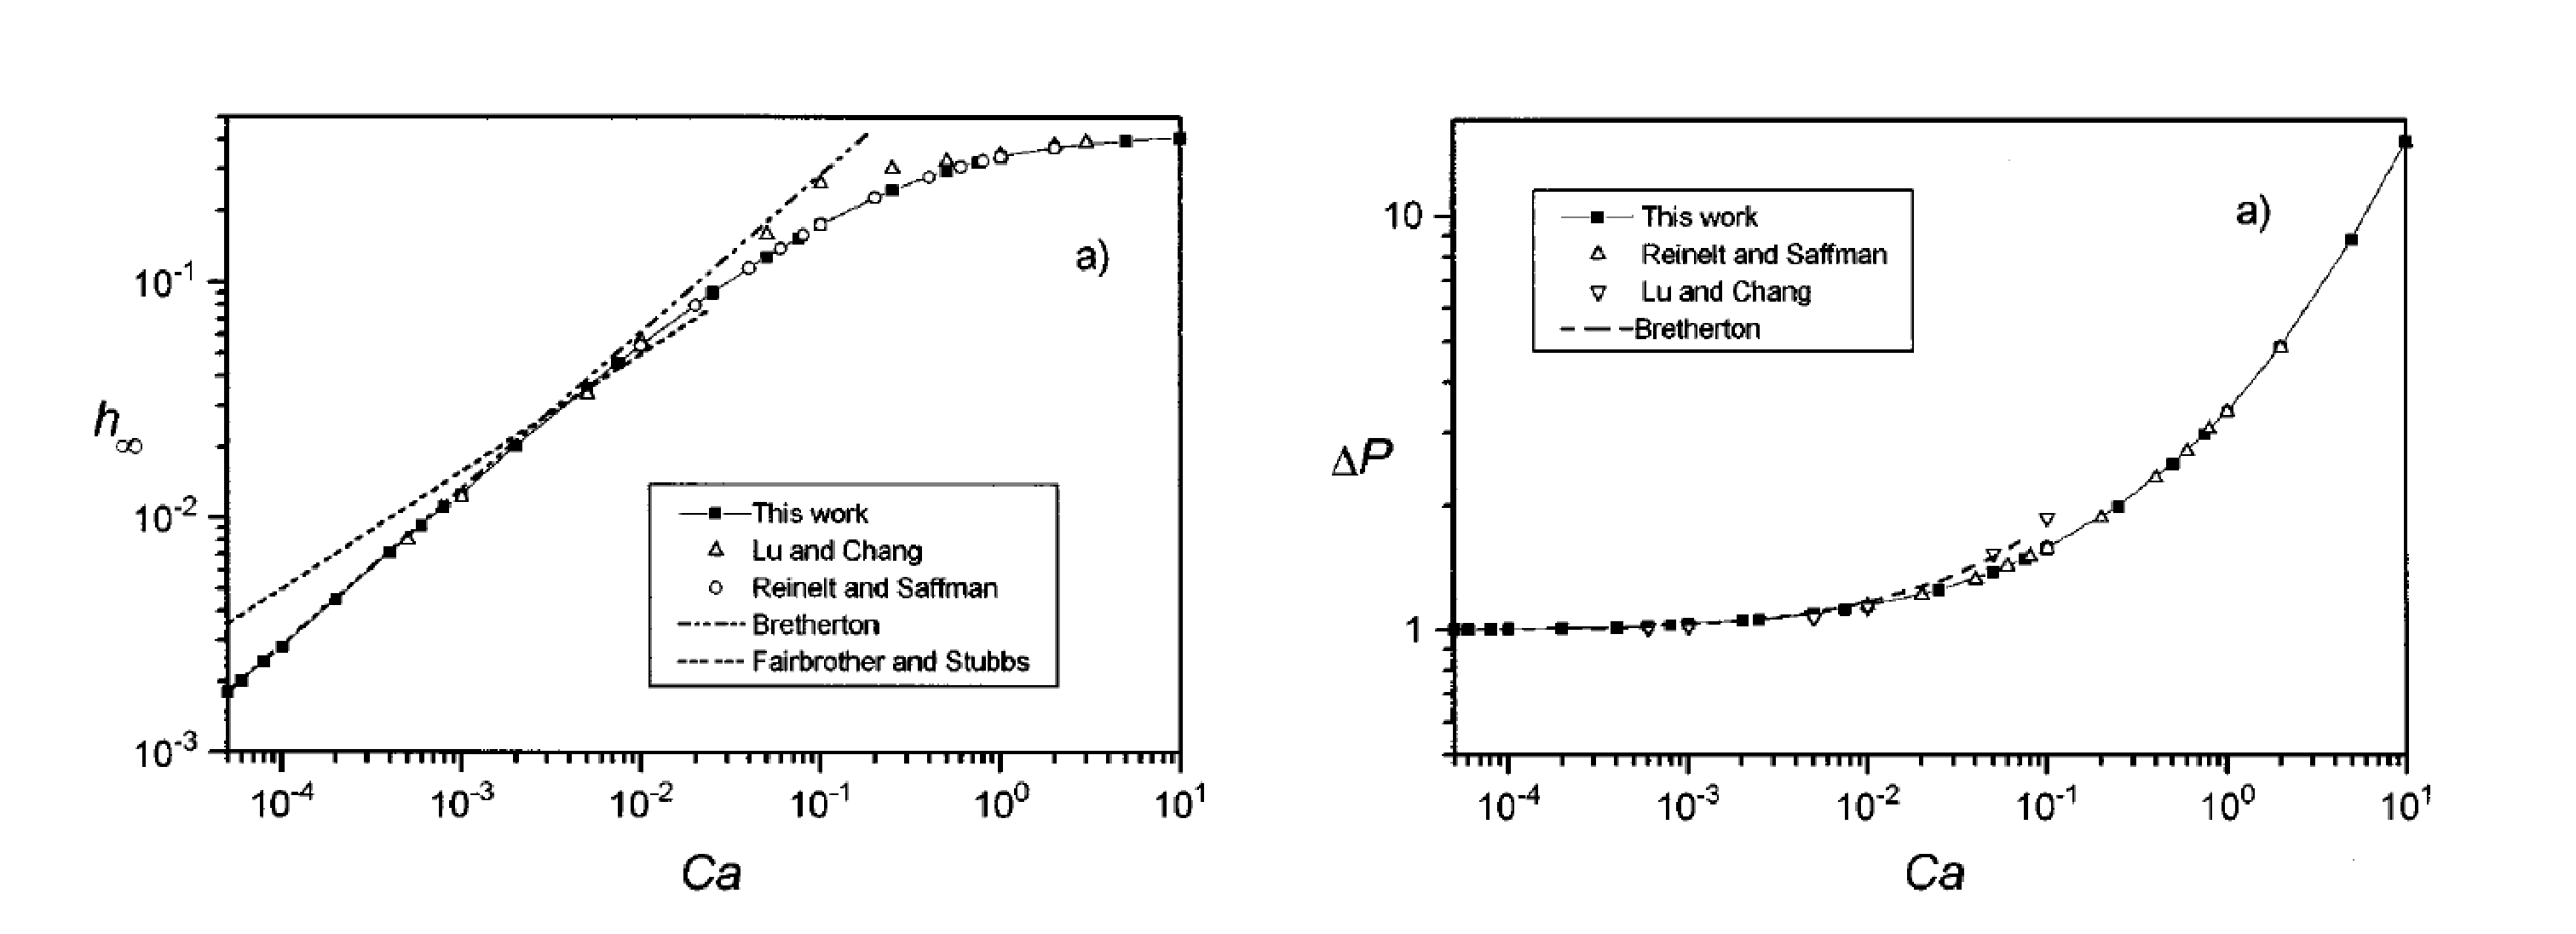
\includegraphics[width=0.97\textwidth]{Figures/giavedoni_planar.eps}
\caption{\citet{giavedoni-numerical} gathered results across the
literature for different Capillary numbers \label{fig:giavedoni:planar}}
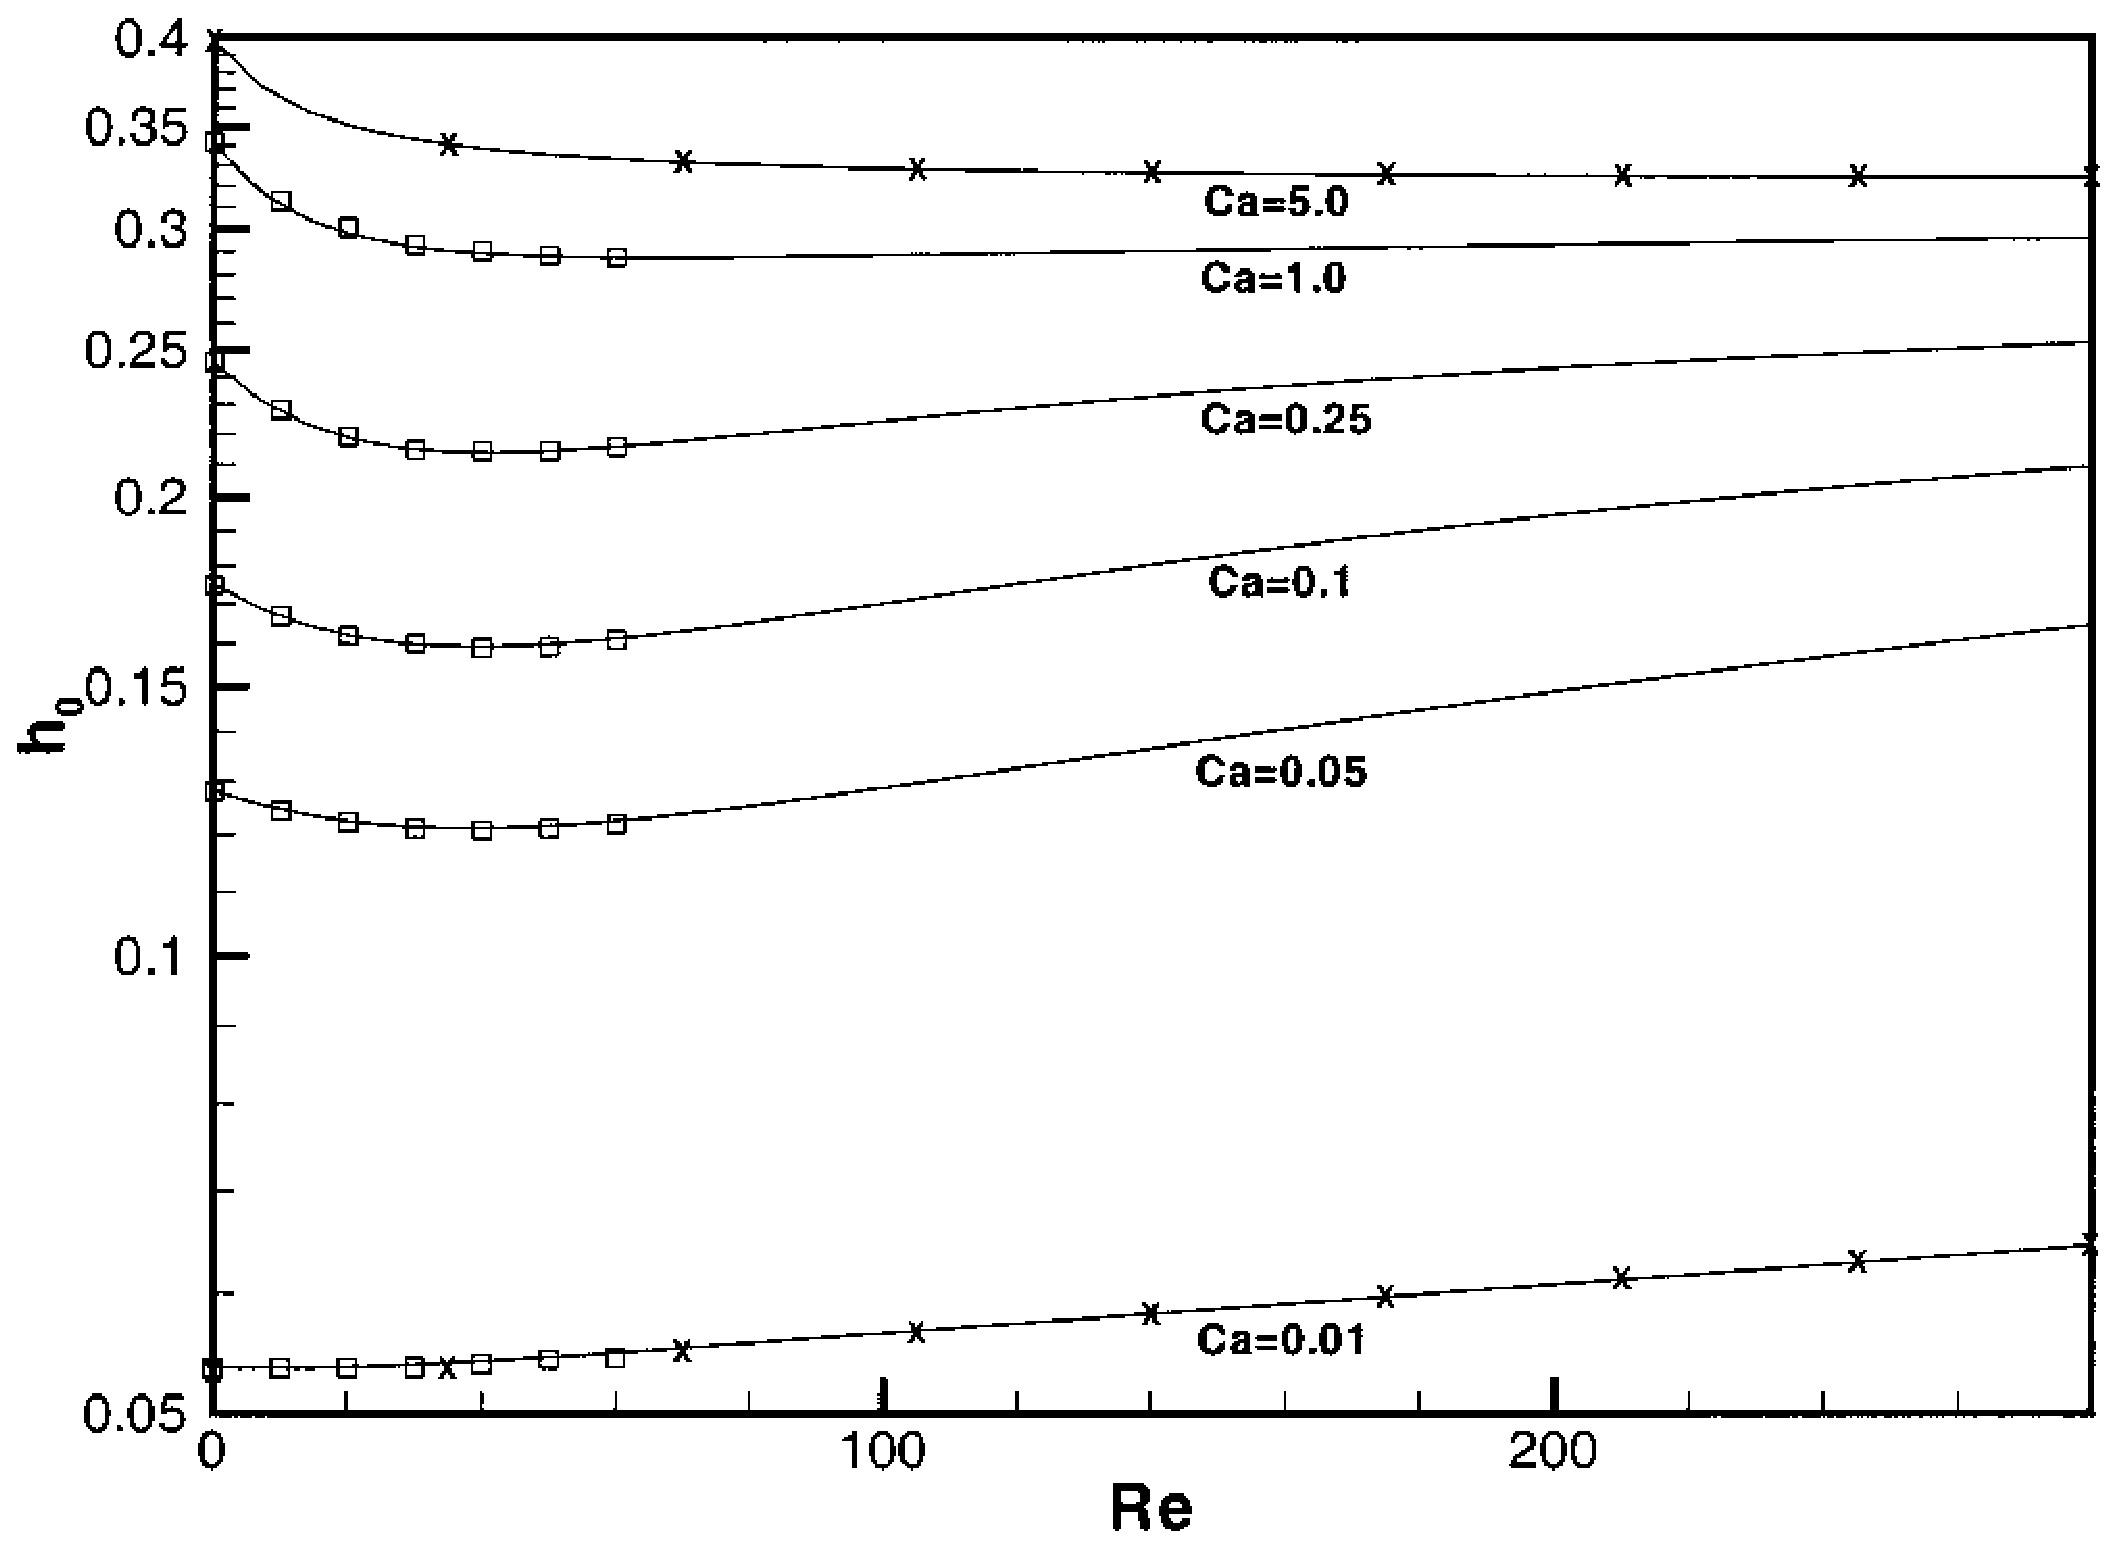
\includegraphics[width=0.97\textwidth]{Figures/heil-planar.eps}
\caption{\citet{heil-bretherton} performed simulations for different ranges of
Capillary numbers and Reynolds numbers. \label{fig:heil:planar}}
\end{figure}

One can see from the Fig. \ref{fig:heil:planar} that the width for the
Capillary number equal to $0.05$ ranges from $0.12$ to $0.15$ while Reynolds
number ranges from $0$ to $300$. This capillary number has moderate film widths
to be resolved with certain accuracy. Let us recalculate all the necessary
parameters:
\begin{equation}
\begin{aligned}
&Ca=0.05\\
&Ca=\frac{U_{bubble} \mu_{liq}}{\gamma}=0.05.
\end{aligned}
\end{equation}
Some parameters are fixed with the model parameters, as surface tension:
\begin{equation}
\gamma=\sqrt{\frac{8 k A}{9}}=\sqrt{\frac{8 0.04 0.04}{9}}=0.037712
\end{equation}
The film width for such small Capillary numbers is taken from
\ref{fig:heil:planar} for Reynolds number $40$ equals to $0.12$. We want to
resolve $12\%$ with $6$ lattice units. Therefore the channel
width is $50$ lattice units. We take the bubble length as $5$ channel widths
and the distance between slugs we take as $2$ bubble lengths. This will give
right away the grid size as $50\mathrm{x}750$. Next step is to calculate the
velocity. The velocity can be calculated from the Capillary number as:
\begin{equation}
U_{bubble}=0.05 \frac{\gamma}{\mu_{liq}}=0.05 \frac{0.037712}{0.6666}=2.82\,
10^{-3},
\end{equation}
where $\mu_{liq}=1/3 (2.5-0.5)=0.6666$. This implies the viscosity ratio to be
equal $R_{\nu}=2/0.2=10$ if we take the relaxation parameter for gas as
$\tau_{gas}=0.7$.
This velocity implies the following pressure gradient calculated from the
Poisuielle flow solution:
\begin{equation}
\begin{aligned}
&\frac{\mathrm{d}P}{\mathrm{d}x}=\frac{8}{Ny^2}\gamma Ca=6.003\,10^{-6}.
\end{aligned}
\end{equation}

Some pictures after $40000$ steps for the gravity driven flow and for different
initialization of bubble width as $Ny-12$, $Ny-20$, $Ny-28$.
\begin{figure}
\includegraphics*[bb=18 350 594 450,width=0.97\textwidth]
{Figures/force_width_6.eps}
\includegraphics*[bb=18 350 594 450,
width=0.97\textwidth]{Figures/force_width_10.eps}
\includegraphics*[bb=18 350 594 450,
width=0.97\textwidth]{Figures/force_width_14.eps}
\caption{The phase plots for different bubble widths as $Ny-12$,$Ny-20$ and
$Ny-28$.}
\end{figure}
\begin{figure}
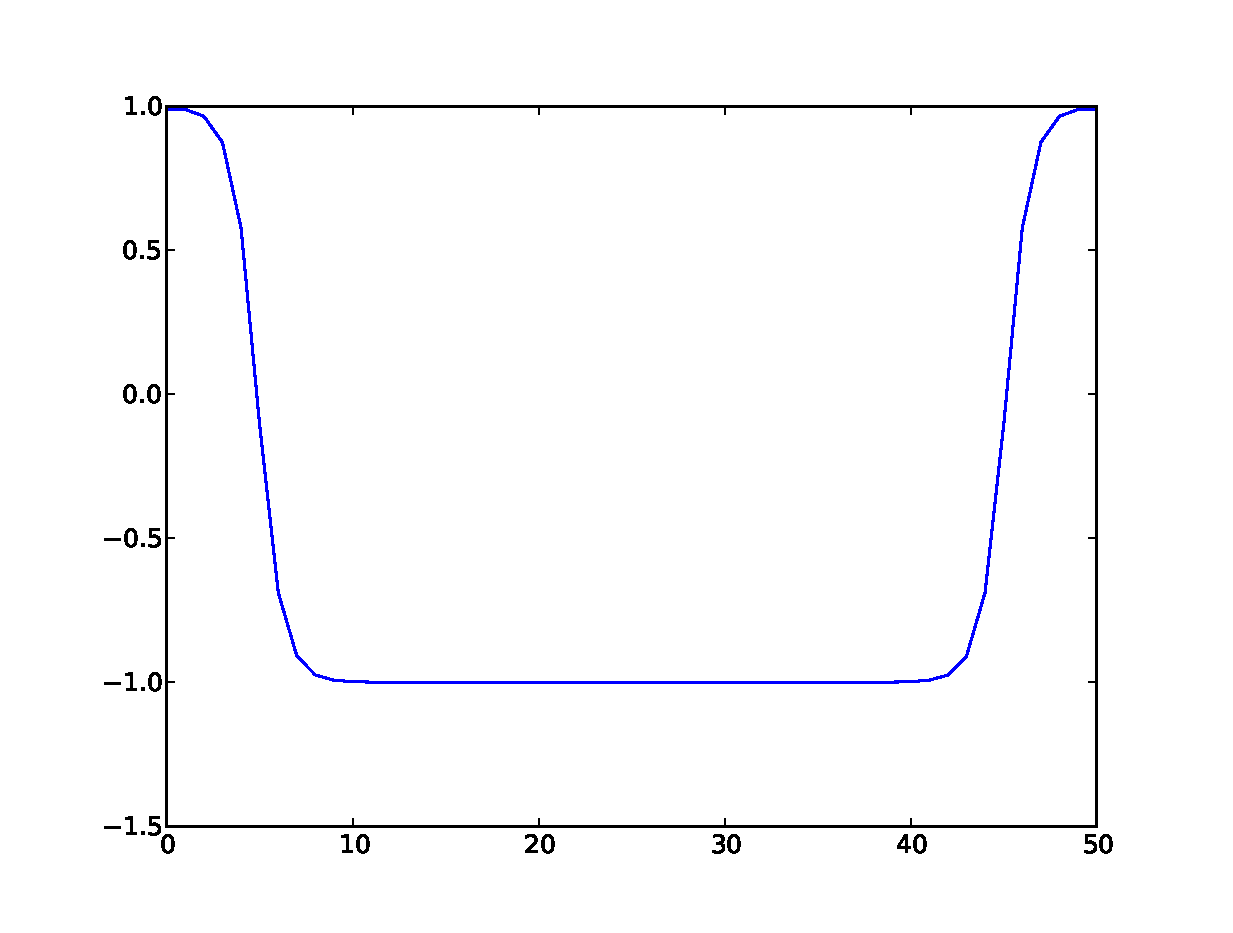
\includegraphics[width=0.47\textwidth]{Figures/plane_force_width_6.eps}
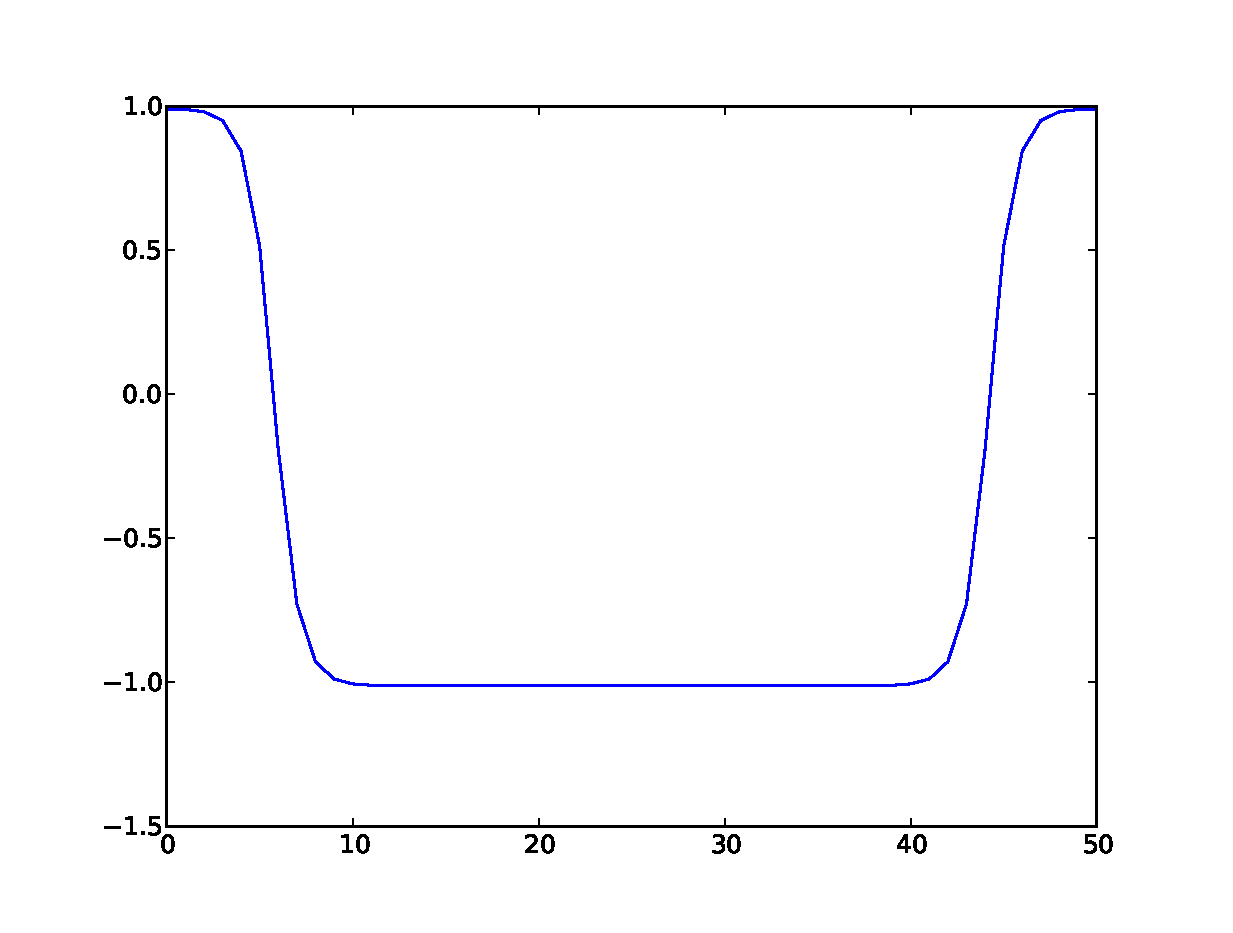
\includegraphics[width=0.47\textwidth]{Figures/plane_force_width_10.eps}
\begin{center}
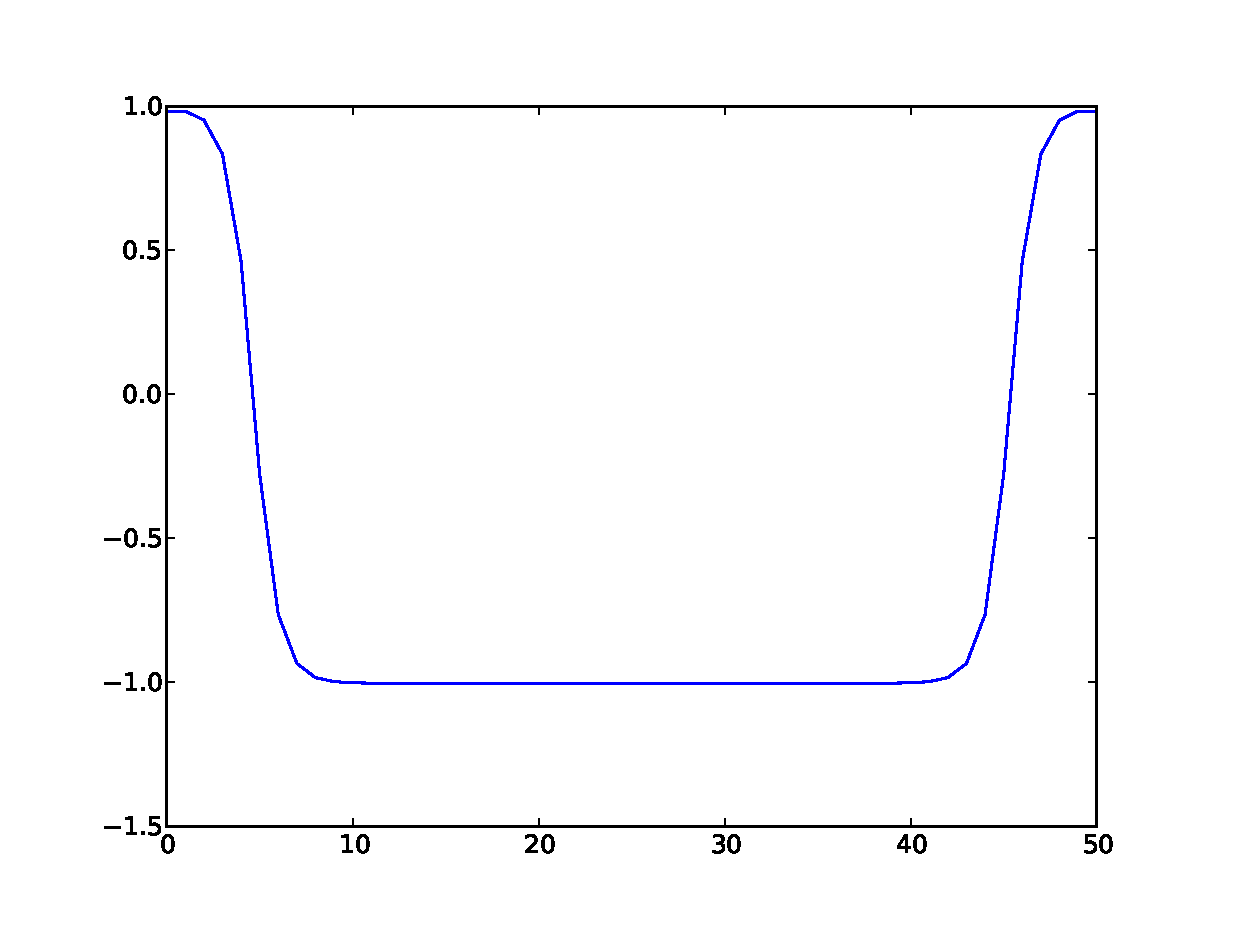
\includegraphics[width=0.47\textwidth]{Figures/plane_force_width_14.eps}
\end{center}
\caption{The phase profiles for different initialization parameters as the
bubble width $Ny-12$,$Ny-20$ and $Ny-28$.
\label{fig:phase:profiles:different:widths:force}}
\end{figure}

One can see from Figures \ref{fig:phase:profiles:different:widths:force} that
the film pattern in the beginning of the slug is almost independent of the
initial conditions and it ranges from 4 to 5 lattice boltzmann units, where the
is taken where the phase field has a value of zero. This preliminary result
justify that lattice Boltzmann method is able to predict the film thickness. 

However, with the smaller initialization of the bubble one can see that the
front meniscus where the film thickness is validated accross is decreasing.
Therefore to be on the safe side one needs to initialize bubbles to be near the
analytical length.

We assumed that the interface thickness should be around $6$ lattice boltzmann
units, but we assume the calculations to be based on the $U_{slug}$ taken from
the simple Poisuille flow velocities. In reality the slug has slippage factor
with with the flow and velocity is slightly bigger than the liquid media. One
can take the velocity of the bubble from the simulations and recalculate all
the necessary lengths. Velocity profiles behind the bubble and in the front
meniscus can be seen in Fig. \ref{fig:velocity:profiles:different:widths:force}
and \ref{fig:velocity:profiles:different:widths:pressure} for the force driven
and pressure difference driven flows, correspondingly. As one can see average
velocity for the bubble and the slug larger than the calculated velocity which
should give larger the film. However, the film width for the planar case is
different and can have another coefficient in front of the proportionality to
$Ca^{2/3}$. Also, the phase gradient is taken as $0$ right now which can have
influence on the measurements as well.
\begin{figure}
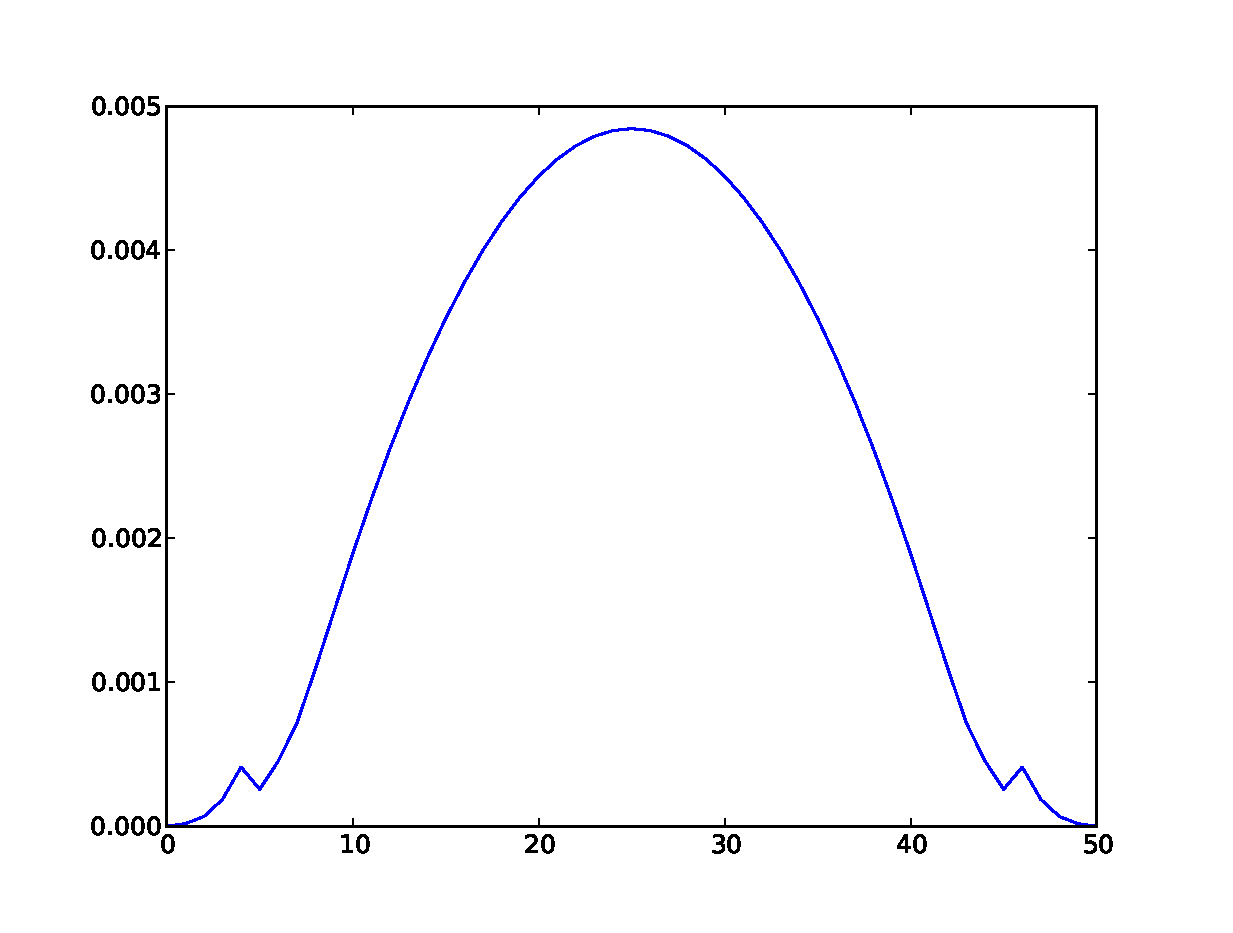
\includegraphics[width=0.47\textwidth]{Figures/vel_bubble_force_width_6.eps}
\hfill
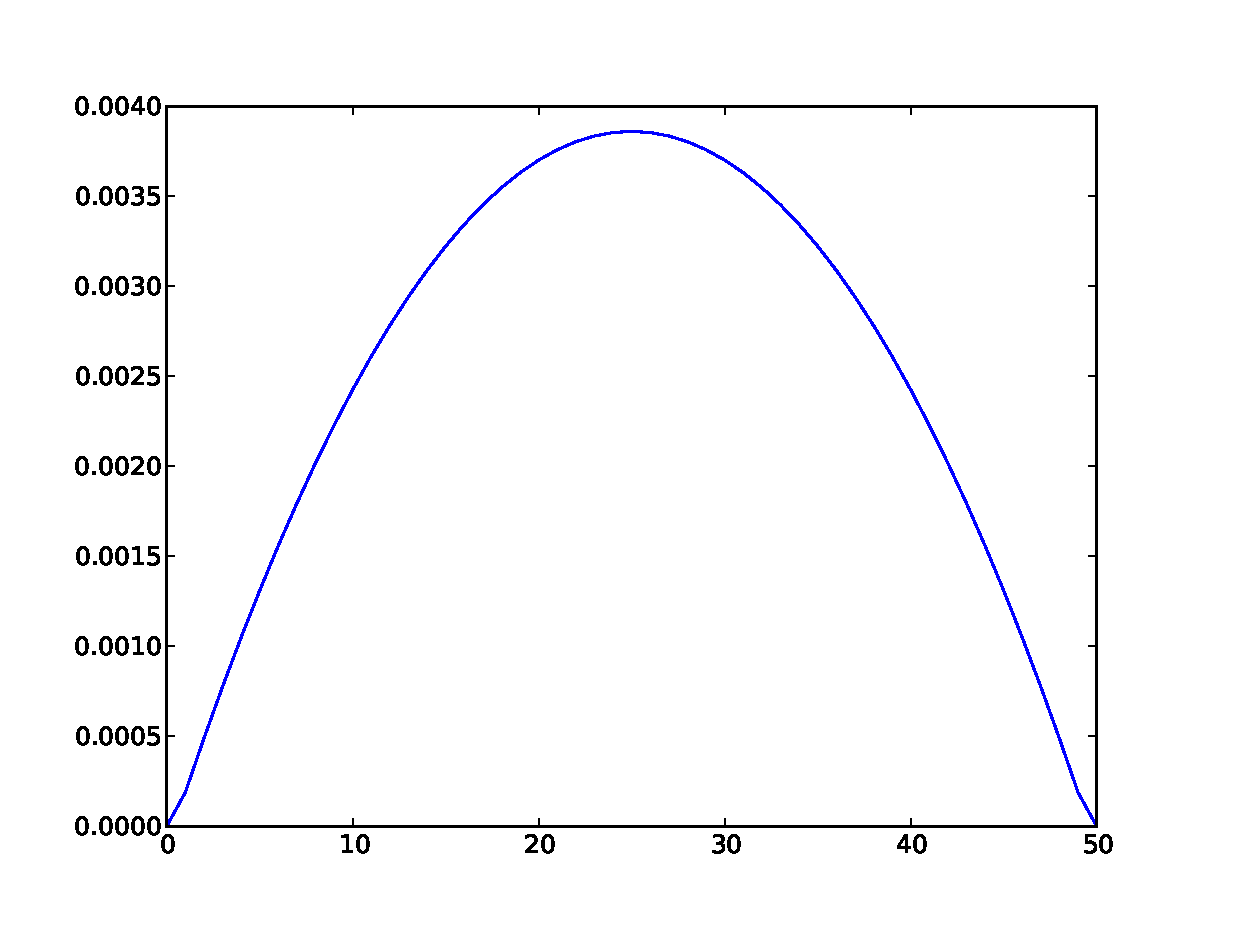
\includegraphics[width=0.47\textwidth]{Figures/vel_bulk_force_width_6.eps}\\
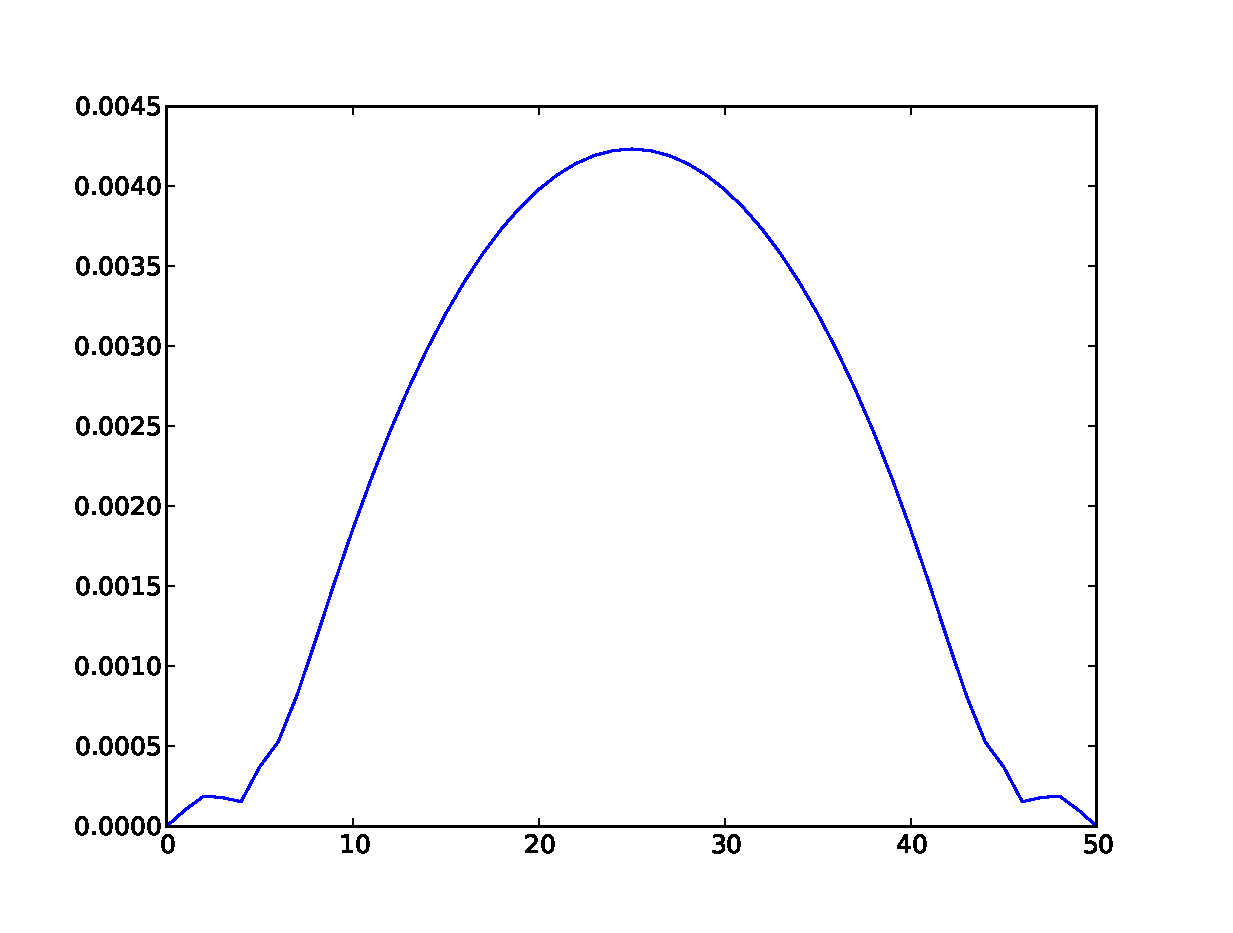
\includegraphics[width=0.47\textwidth]{Figures/vel_bubble_force_width_10.eps}
\hfill
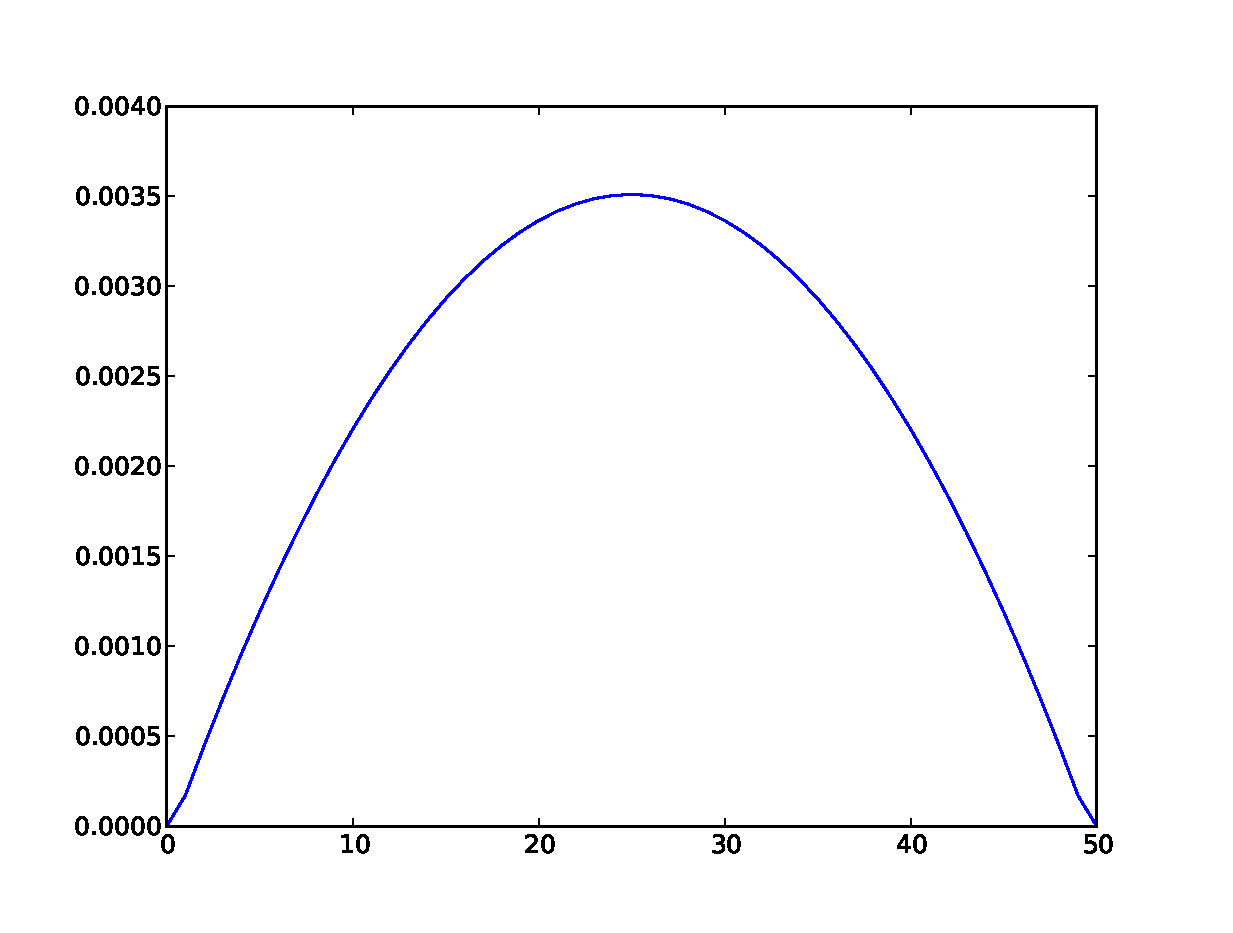
\includegraphics[width=0.47\textwidth]{Figures/vel_bulk_force_width_10.eps}\\
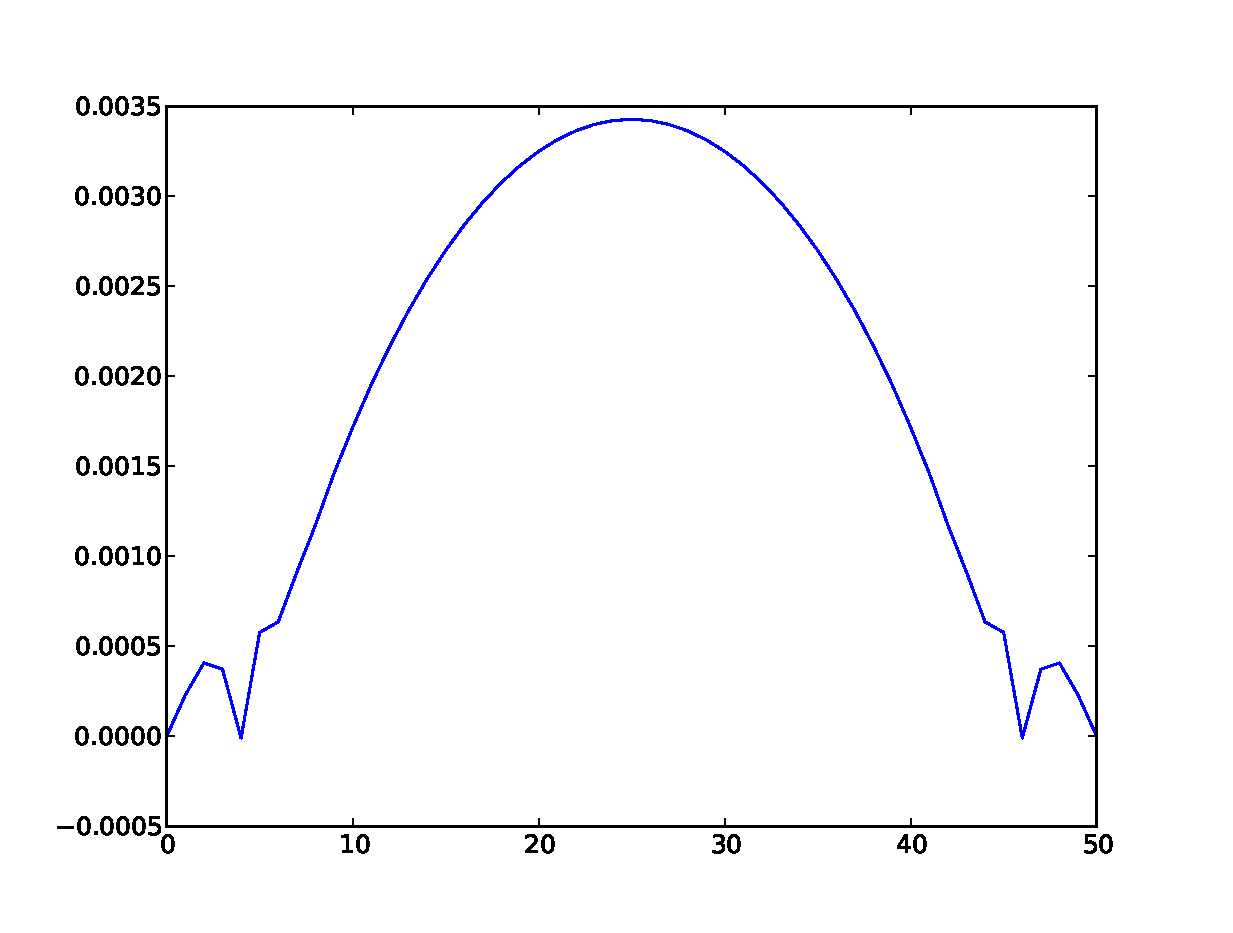
\includegraphics[width=0.47\textwidth]{Figures/vel_bubble_force_width_14.eps}
\hfill
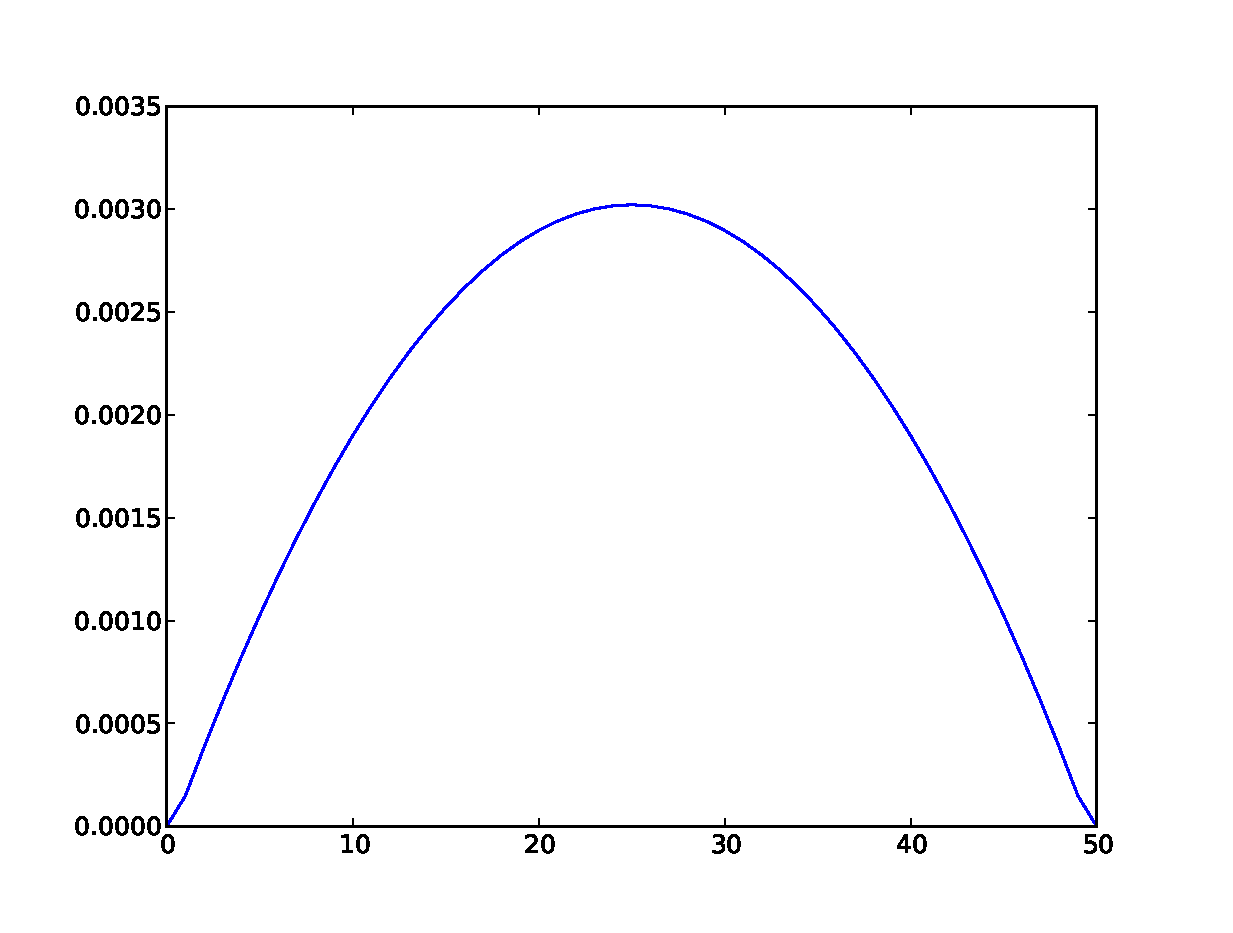
\includegraphics[width=0.47\textwidth]{Figures/vel_bulk_force_width_14.eps}\\
\caption{The velocity profiles in bulk and bubble for different initialization
parameters as the
bubble width $Ny-12$,$Ny-20$ and $Ny-28$.
\label{fig:velocity:profiles:different:widths:force}}
\end{figure}

While the shapes of droplets are different for the force and pressure
difference driven flows the velocity profiles show that the force driven bubble
move faster than in the case of pressure difference driven flow:
\begin{figure}
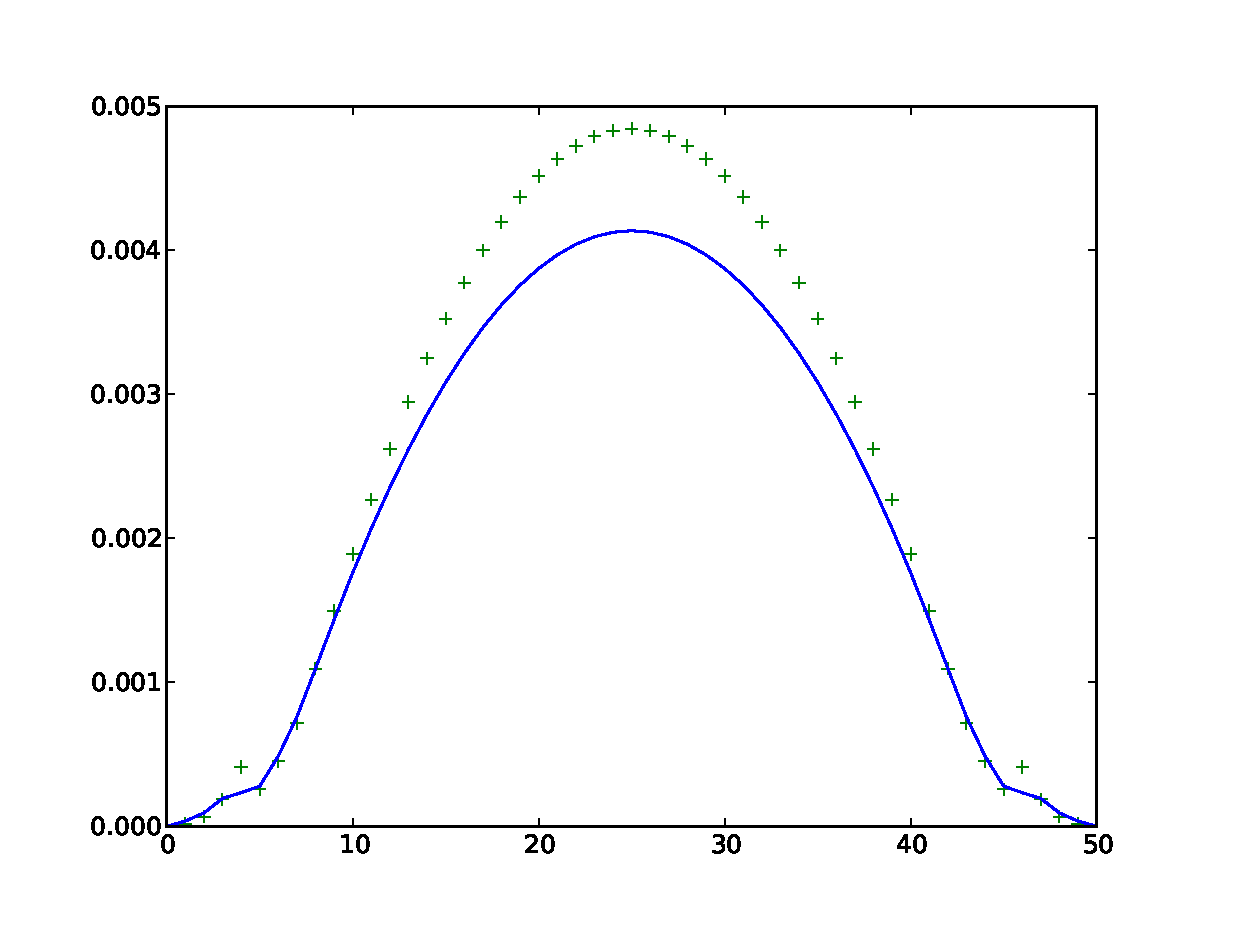
\includegraphics[width=0.47\textwidth]{Figures/vel_comparison_width_6.eps}
\hfill
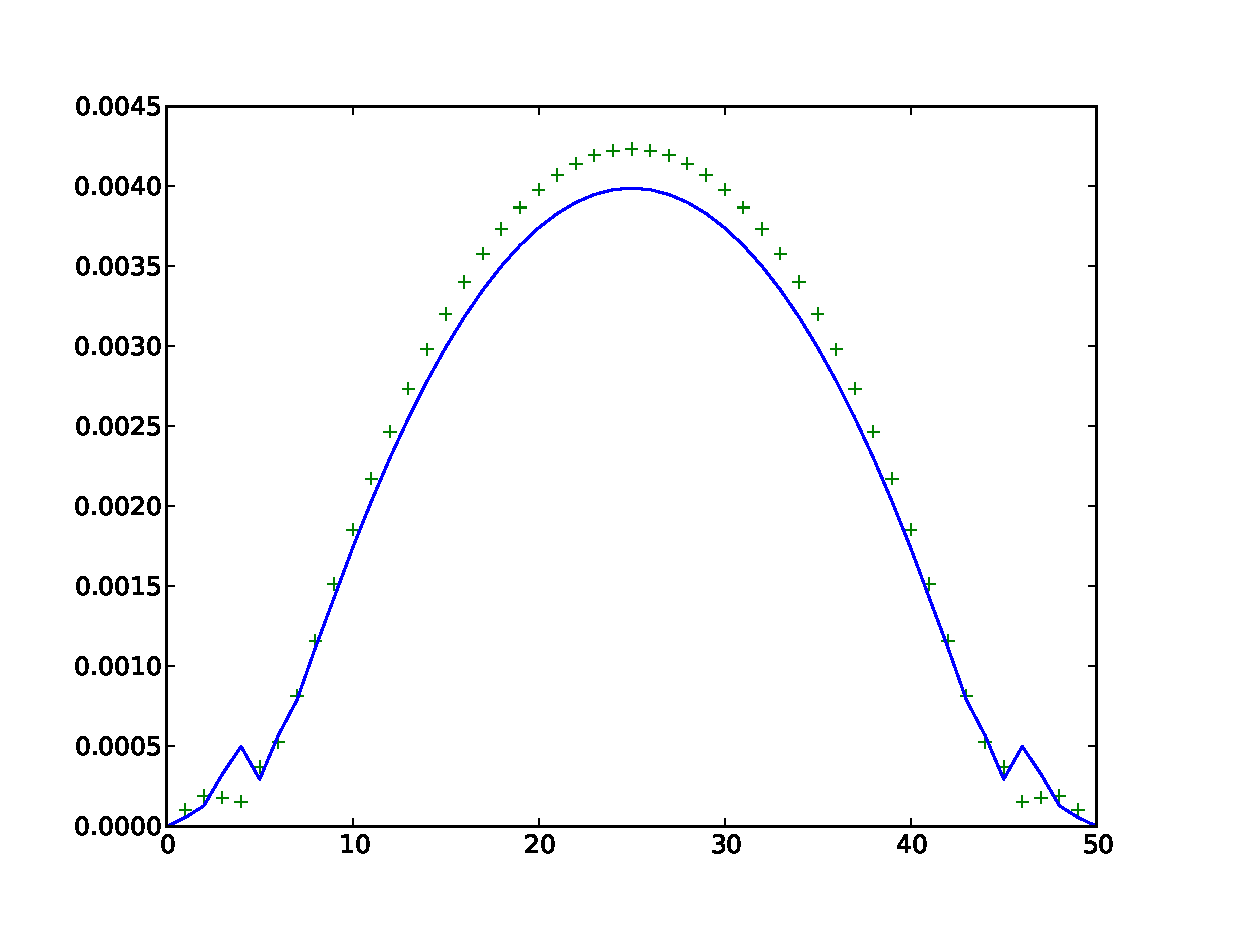
\includegraphics[width=0.47\textwidth]{Figures/vel_comparison_width_10.eps}
\\
\begin{center}
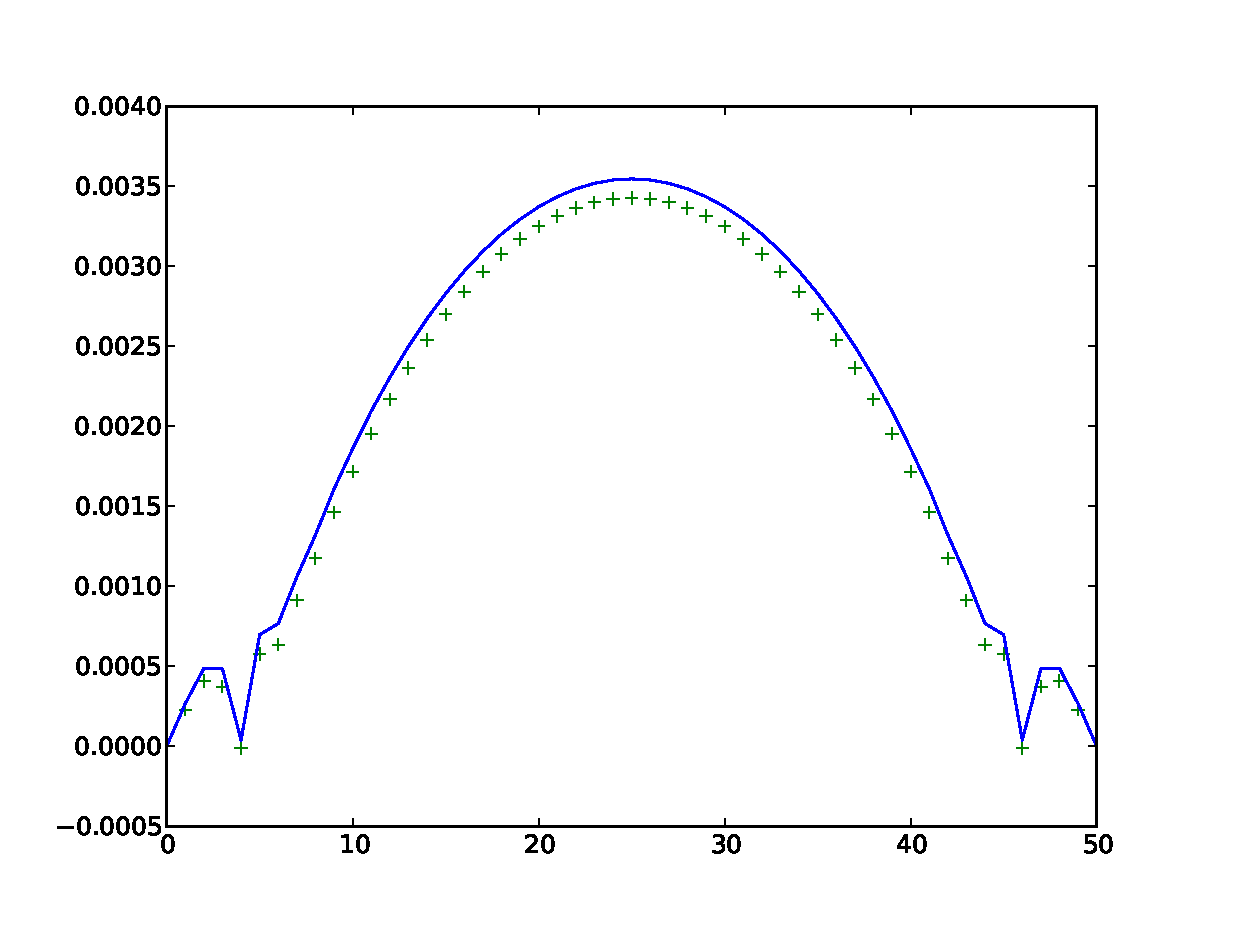
\includegraphics[width=0.47\textwidth]{Figures/vel_comparison_width_14.eps}\\
\end{center}
\caption{Comparison between velocity bubble
profiles.\label{fig:velocity:comparison:different:widths}}
\end{figure}

Note that in the case of pressure driven flows the termination bulk and bubble
velocity have more consistent behavior and the values are not different too
much. That is one of the reasons why in the case of the force driven flows the
width has a bit different values depending on the initialization procedure. 


\subsection{Grid refinement}
To examine the interface width we performed grid refinement for both force and
pressure difference driven flows. To avoid the effects of rear and front
menisci the problem is initialized with the film width occupying $12$ percent
of the channel height. All other parameters are kept the same, that includes
keeping the same Capillary number and viscosities ratio. Therefore the
following parameters were utilized: $Ny=51,100,149,198$,corresponding to the
effective channels widths as $H_{eff}=49,98,147,196$, $Nx=736,1471,2206,2941=15
H_{eff}$. It is easy to check
that keeping all liquid viscosities the same yields the following to be
constant while doing the grid refinement
$H^2\frac{\mathrm{d}P}{\mathrm{d}x}=Ny^2\frac{\mathrm{d}P}{\mathrm{d}x}=Const$.
The results for the force driven flows velocity phase profiles are shown in
Fig. \ref{fig:grid:profiles}. The corresponding ratios to the effective channel
width (without bounce-back nodes) is as $0.0809472165313,
0.0708111118485, 0.0678483852412, 0.0664499716904$. One can see
that for the channel widths as $149,198$, the results are convergent. The
velocities in the center of the bubble are $0.004176469553,
0.00401004133, 0.003969909065, 0.00394134433$, which corresponds
to the $Ca=\frac{\mu_{liq} U_{bubble}}{\gamma}=\frac{\frac{2}{3}\,
0.0045}{0.03771}=0.069$, which is slightly higher when for the assumed
profile. However, if we define Capillary number through the velocity of the
slug, then the Capillary number will have another value. The velocities of the
slug are $0.003411444831,0.003412693869,0.003420338754,0.003425757312$ and
Capillary number defined through these velocities is $0.0602$. Those numbers
are adequate if we assume that the results presented in
Fig.\ref{fig:giavedoni:planar} and Fig. \ref{fig:heil:planar} correspond to the
half of the channel but not the whole channel. 

Let us calculate to which extent we need to refine the interface to obtain
convergent results. The interface itself occupies approximately $5 \xi$, where
$\xi=\sqrt{k/A}=1$. This interface width divided to the effective channel width
($5\xi/H_{eff}$) is as follows $0.102,0.051,0.034,0.025$ for the given
$H_{eff}$. However, the interface width needs to be takes as the ratio with the
film width which we want to resolve, this ratio $5\xi/H_{film}$ is as follows
$1.2605,  0.7205,  0.501,  0.3839$. In reality this number is
a bit overestimated as the interface doesn't fill the influence of the wall and
it maintains all the macroscopic parameters jumps. Therefore, one needs to
resolve the interface as $40\%$ of the expected film width.
\begin{figure}
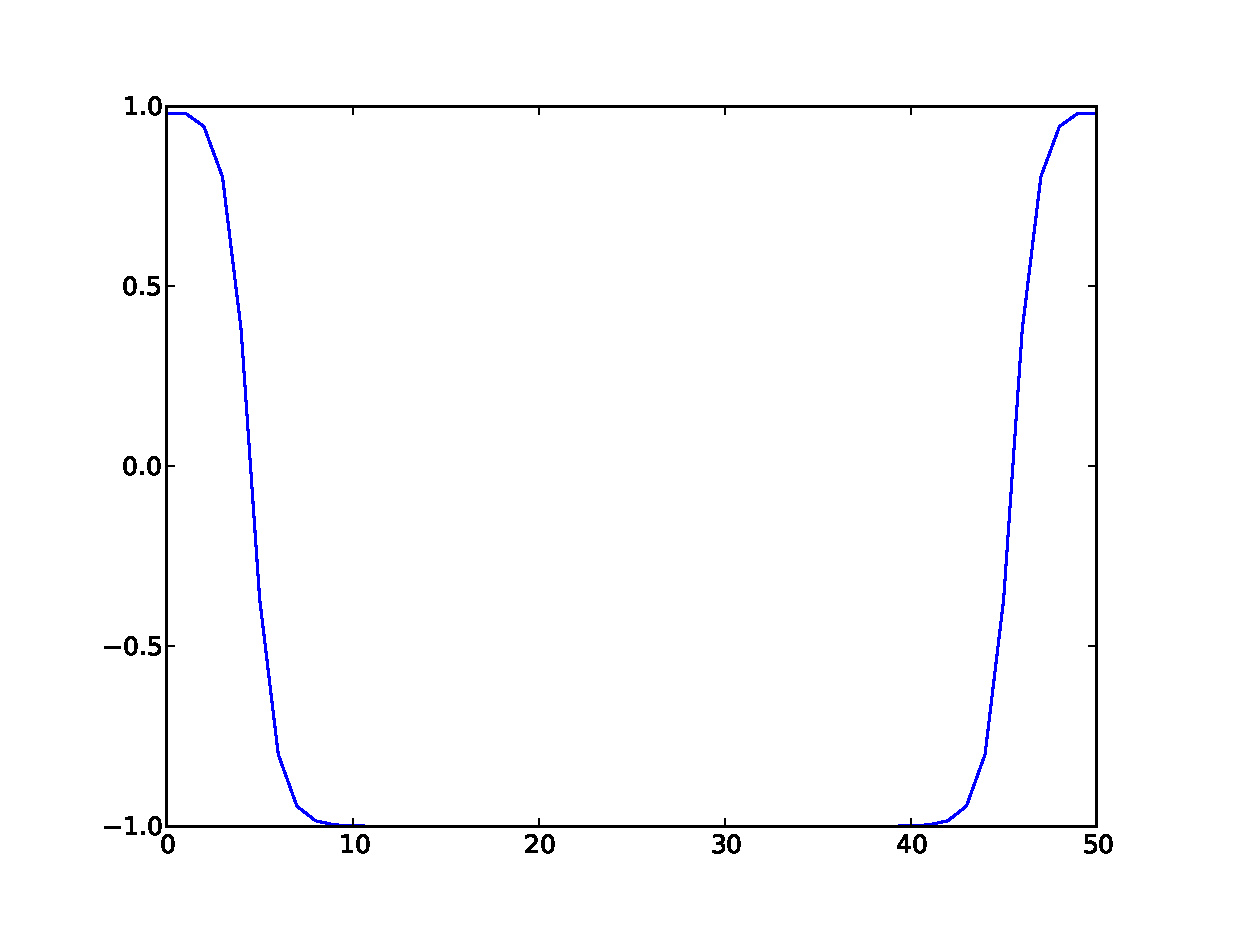
\includegraphics[width=0.47\textwidth]{Figures/grid_phase_prof_49.eps}\hfill
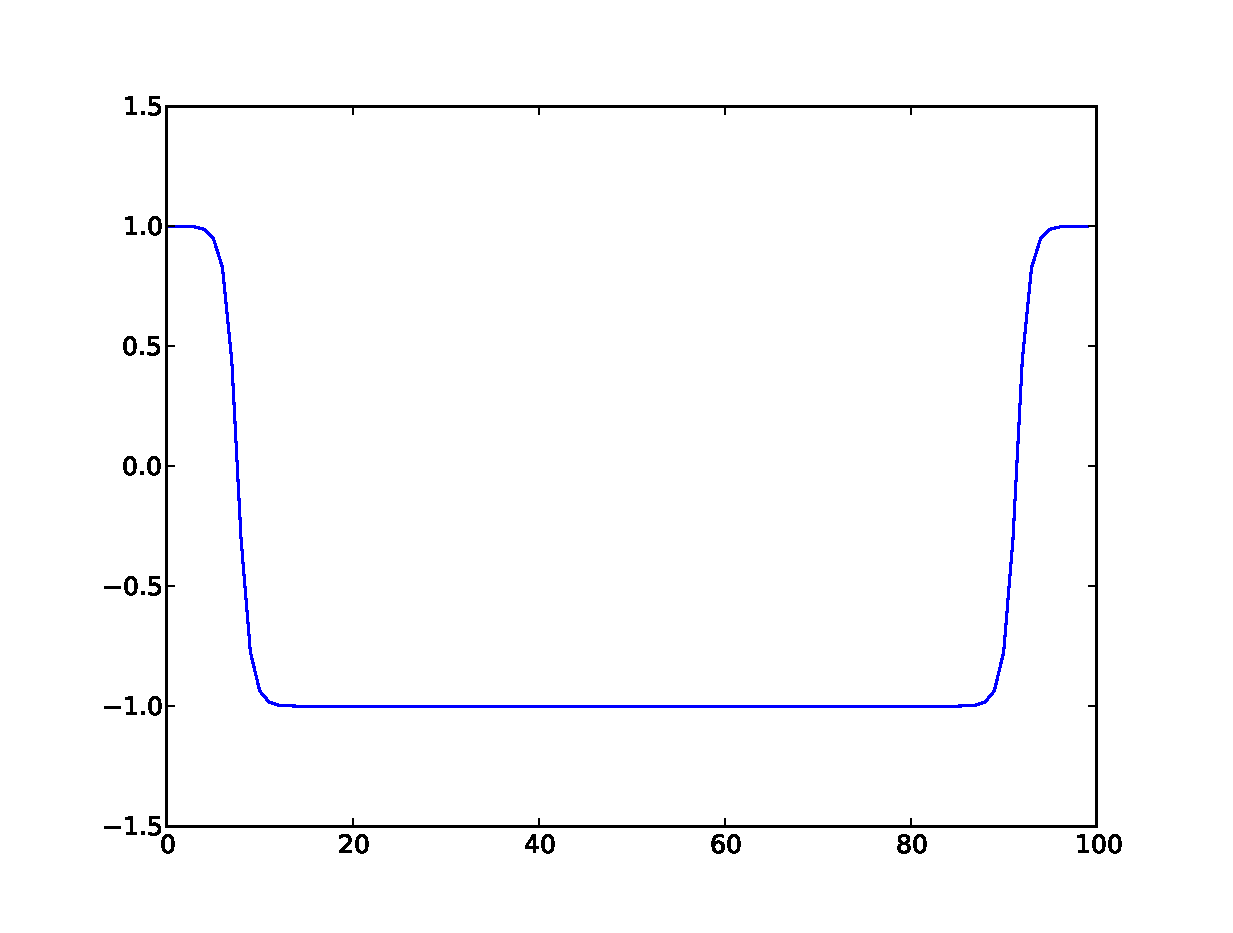
\includegraphics[width=0.47\textwidth]{Figures/grid_phase_prof_98.eps}\\
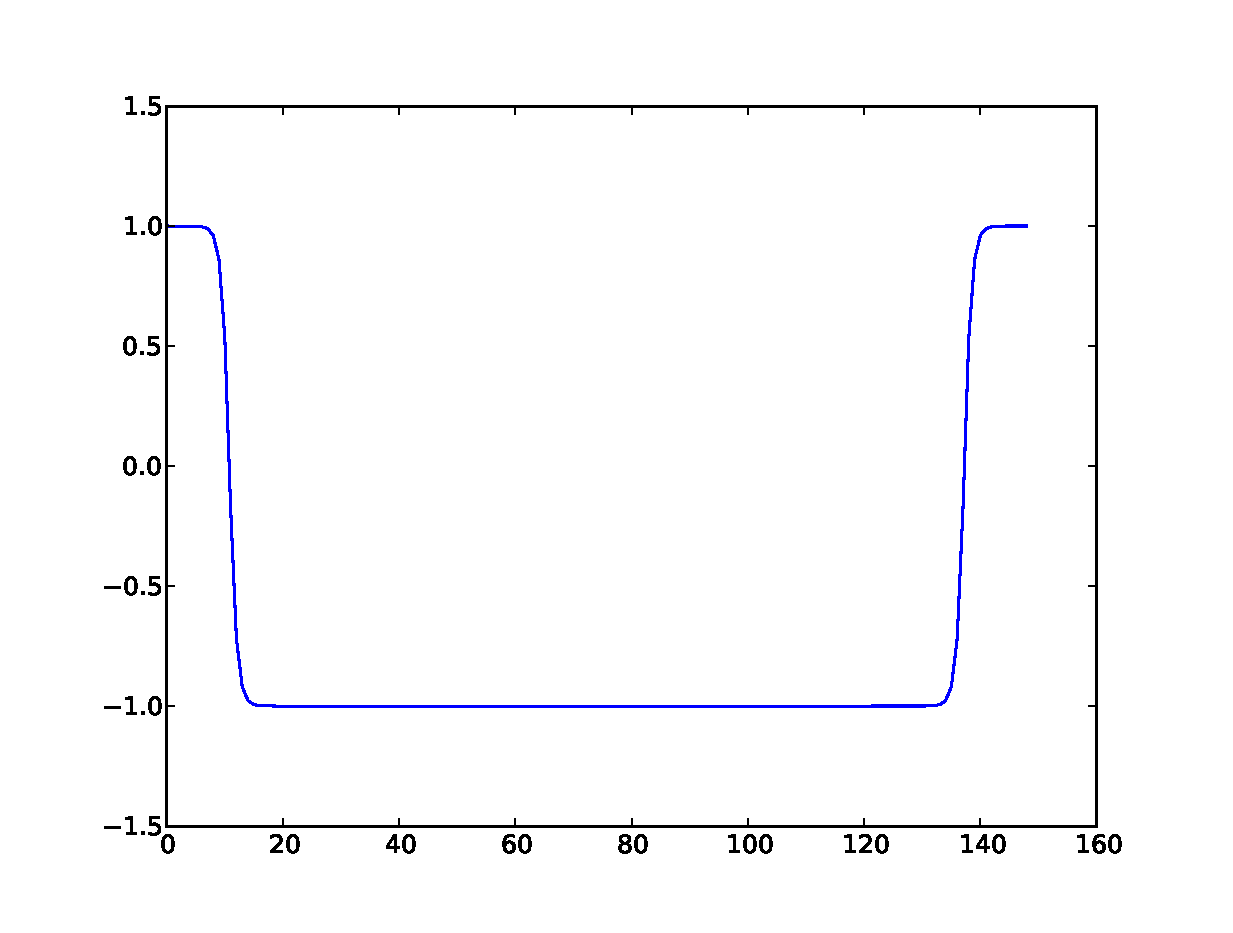
\includegraphics[width=0.47\textwidth]{Figures/grid_phase_prof_147.eps}\hfill
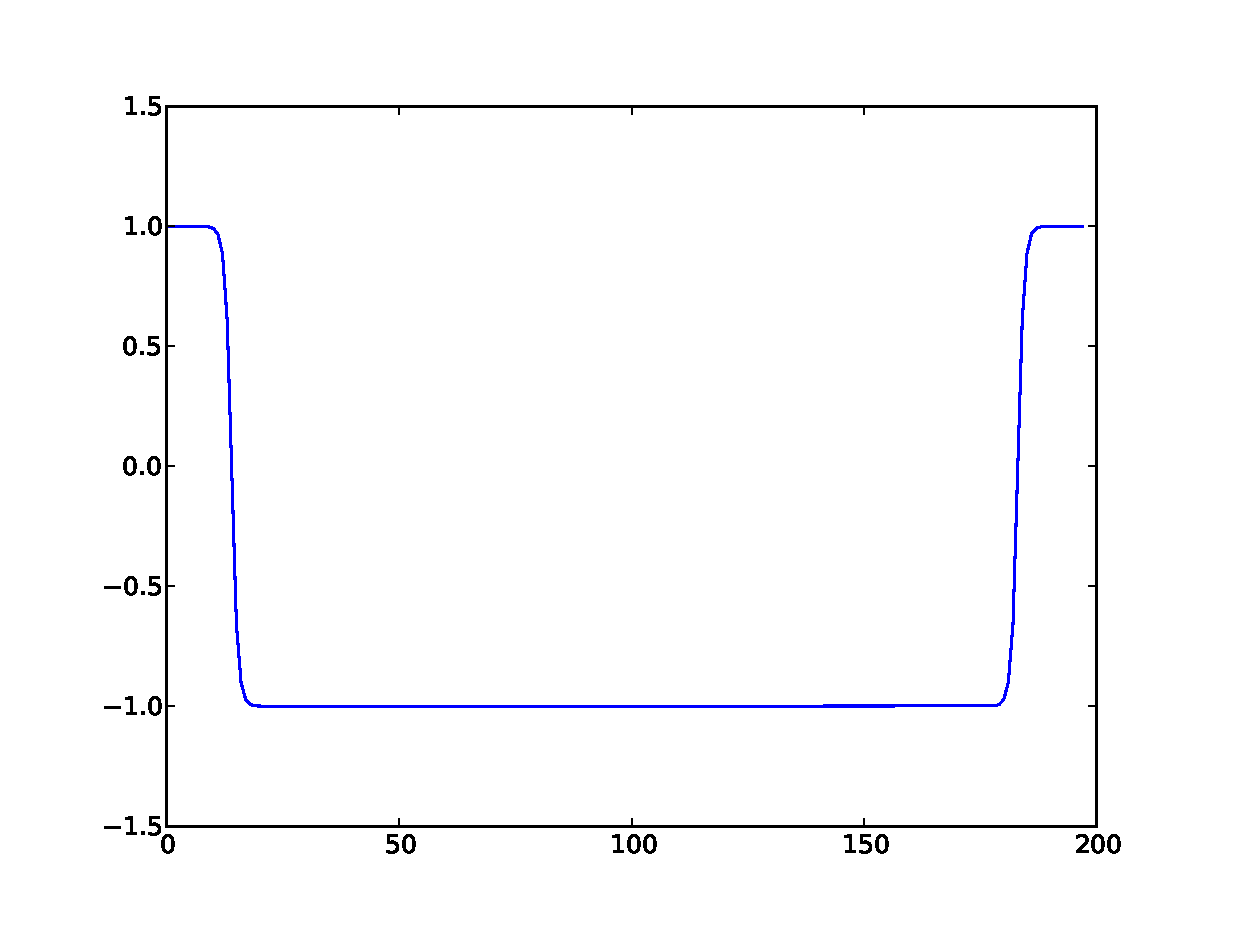
\includegraphics[width=0.47\textwidth]{Figures/grid_phase_prof_196.eps}\\
\caption{Grid refined profiles for the effictive channel widths
$H_{eff}=49,98,147,196$.\label{fig:grid:profiles}}
\end{figure}

{\color{red} The next step is to perform calculations for different Capillary
numbers to restore necessary characteristics as it's seen in Fig.
\ref{fig:giavedoni:planar} and \ref{fig:heil:planar}. Also note that grid
refinement is done for the gravity driven flows, which can have pretty
different characteristics in comparison with pressure simulations (unstable
for the grid refinement - need to adjust parameters)}.

\section{Capillary number region}
This section is devoted to the study of different Capillary number. We refer to
grid refinement section where we obtained that the interface width should be
at most $40$ percent of the interface width. For the benchmark results we
suggest the following Capillary numbers as:
\begin{equation}
0.03,0.05,0.08,0.1,0.2,0.4,0.6,0.8,1.0
\end{equation}
The corresponding approximate film widths from \cite{giavedoni-numerical} are as
follows (we take the half width as it's done in the grid refinement section):
$0.04,0.06,0.08,0.1,0.12,0.13,0.15$. $5$ lattice boltzmann units occupy
$40\%$ of the interface thickness. Therefore the grid size should be as
following $314\mathrm{x}4681$,$210\mathrm{x}3121$,
$158\mathrm{x}2341$, $127\mathrm{x}1876$, $106\mathrm{x}1561$,
$98\mathrm{x}1441$,$85\mathrm{x}1246$. 

To utilize previous results to properly initialize simulations to run one need
to do some modifications. The result is that for the grid with $H_{eff}=196$ we
obtained the film width as $0.0685$ and velocity in the center of the bubble as
$0.0045$. The force gradient was $6\, 10^{-6} /16$. The predicted Capillary
number was $0.05$ and the actual one is $0.0795$. But we performed simulations
according the assumed value of $0.05$. Let us perform some correlations to
calculate how the system needs to be initialized. 
\begin{equation}
\begin{aligned}
&Ca_{lit} \propto U_{slug}\\
&U_{slug} \propto \frac{\mathrm{d}P}{\mathrm{d}x} Ny^2 
&Ca_{lit} \propto \frac{\mathrm{d}P}{\mathrm{d} x} Ny^2 \text{ or }\\
\frac{\mathrm{d}P}{\mathrm{d} x} \propto \frac{Ca_{lit}}{Ny^2}
\end{aligned}
\end{equation}
Therefore the initialized consistent pressure gradients can be taken from
previous consistent simulations:
\begin{equation}
\frac{\mathrm{d}P}{\mathrm{d} x}=6\,10^{-6}/16 \frac{Ca_{literature}}{0.05}
\frac{196^2}{Ny^2}=0.28812 \frac{Ca_{literature}}{Ny^2}
\end{equation}
Note that $Ny$ is calculated through the expected resolution of the interface
in comparison with the interface thickness which itself is based on
Capillary number simulations. In terms of time the steady state succesfull
simulation for the grid $196$ was obtained after $200,000$ steps. The physical
time is as follows:
\begin{equation}
\begin{aligned}
&\Delta t=\frac{U_{slug,LB} \Delta X}{U_{phys}} \propto \frac{1}{Ny}\\
&N_{iter}=200,000 \frac{Ny}{196}\approx 1020 Ny\\
&N_{output}=51 Ny\\
\end{aligned}
\end{equation}

Steady simulations were obtained for the following Capillary numbers
$0.03,0.05,0.08,0.1$ with the film thicknesses as
$0.0337433850478, 0.063192148642, 0.0799078589211, 0.0891674460655$ which are
quite close to the predicted one $0.04,0.06,0.08,0.1$. The thing is to identify
the Capillary numbers associated with those numbers. The velocity in the
centers are $0.00209258774,0.003826643811,0.006506324324,0.008333889077$. The
Capillary numbers associated with these velocities are $0.036992074529545796, 
0.067646144698590829,0.1150166512524845,0.14732373700007995$, which again a bit
overpredictive but consistent. The bulk liquid velocities for the simulation
are $0.001947507726,0.003364703007,0.005483194352,0.00687516499$. The capillary
numbers associated with those velocities are slightly less than with the bubble
are as follows:$0.034427397986694822, 0.059480107823211698,
0.096930097721574432, 0.12153689465513355$. We can define the average capillary
number defined through the bubble capillary and slug capillaries numbers as
$Ca_{aver}=\frac{Ca_{bubble}+Ca_{slug}}{2}$. The fig.
\ref{fig:capillary:simple} represents the thickness against the Capillary
number which mimics the curve behavior for the Capillary number dependance as
indicated in Fig. \ref{fig:giavedoni:planar}.
\begin{figure}
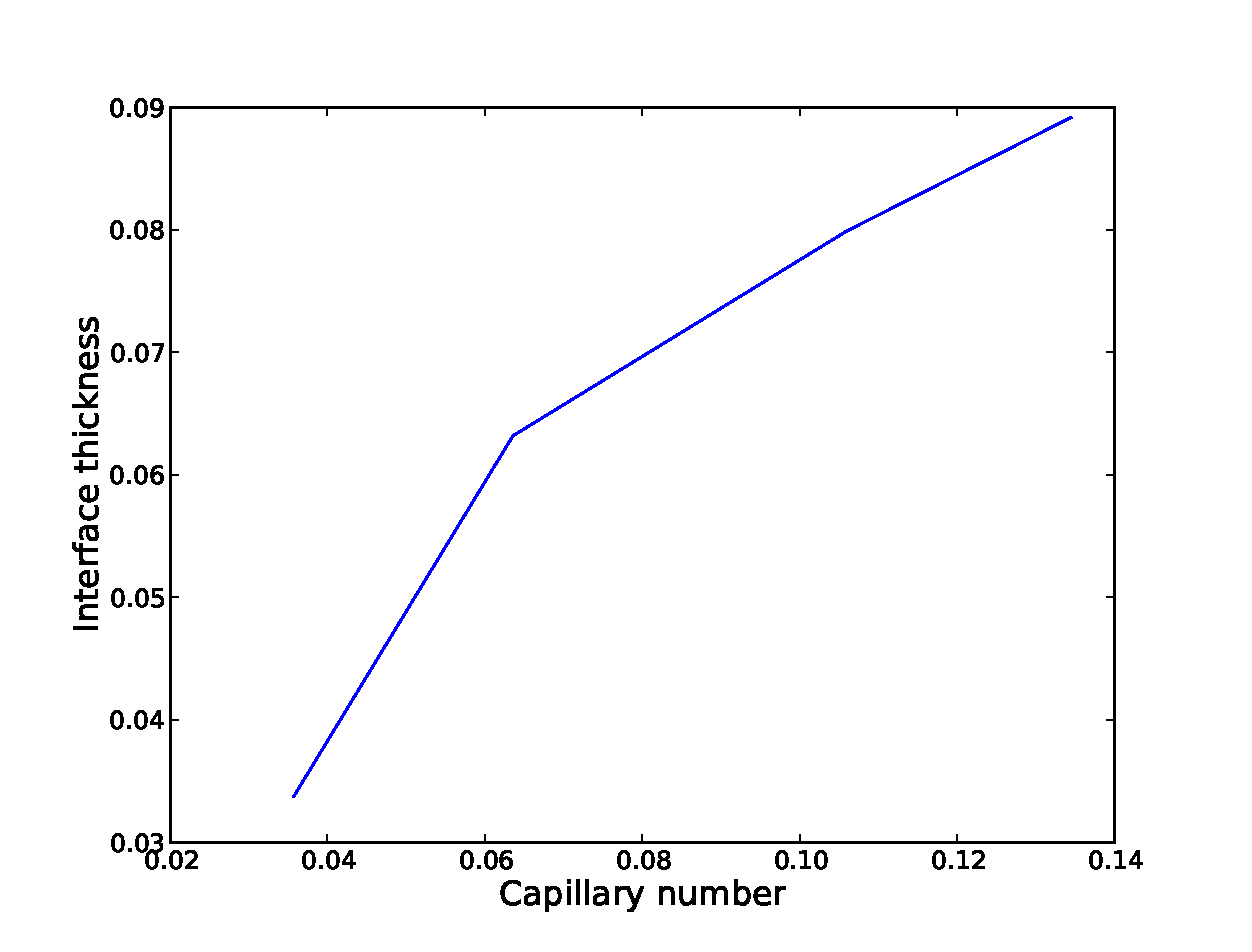
\includegraphics[width=0.47\textwidth]{Figures/capillary_thickness_simple.eps}
\hfill
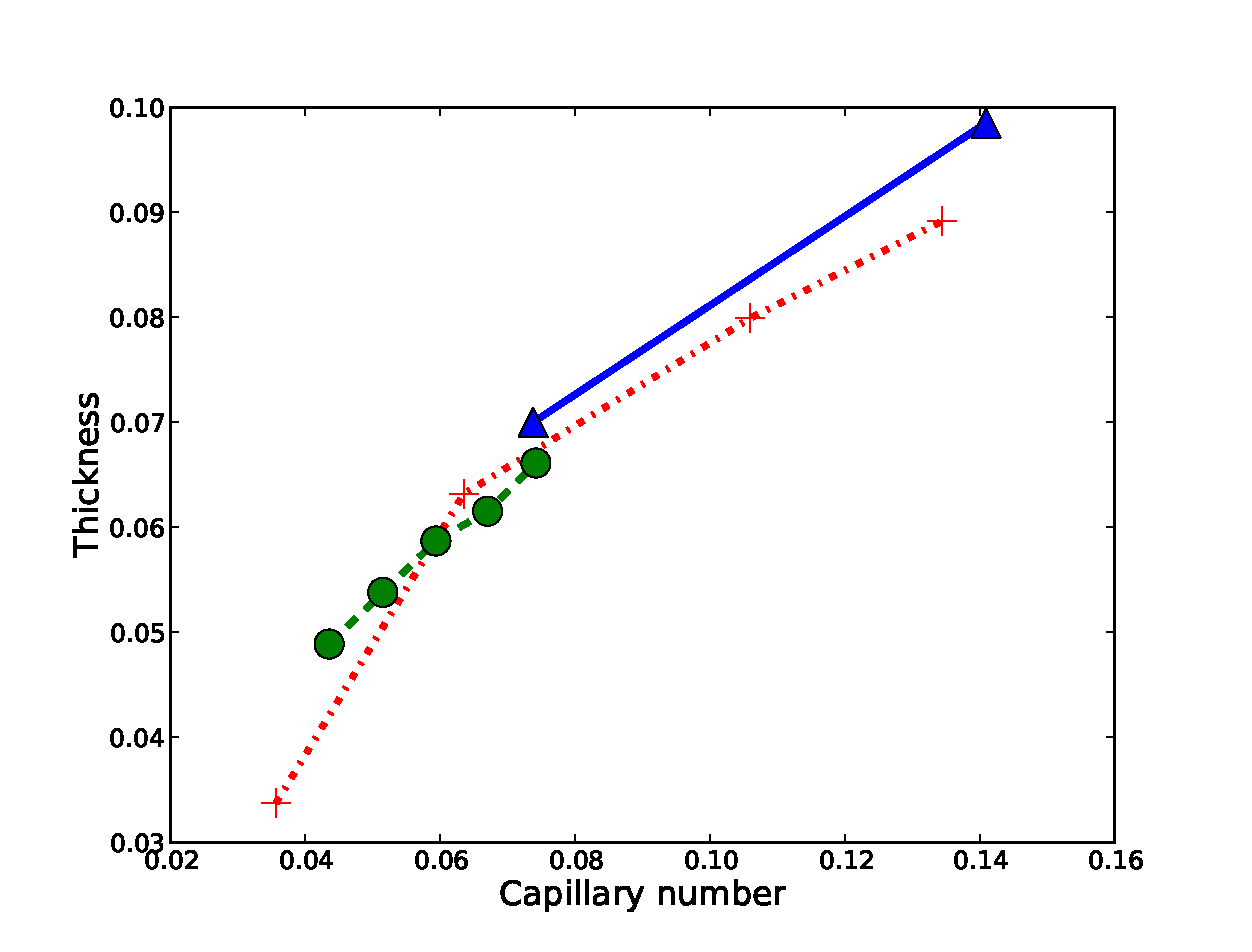
\includegraphics[width=0.47\textwidth]{Figures/capillary_range.eps}
\caption{Thickness versus the capillary number for different scalings based on
the average capillary number. \label{fig:capillary:simple}}
\end{figure}
 
\subsection{The influence of the force}
\begin{description}
 \item 
On the grid $198\mathrm{x}2941$ and the initial film width as $20$ units
the
influence of the force is studied. $16$ different values of force are examined,
which have the following expression $\frac{0.000006}{16} i$, where $i=1 \dots
16$. The system is allowed to come to the equilibrium after $200,000$ steps. The
goal is to study the influence of the force on the velocity and therefore the
capillary number. Unfortunately in the first case only a few simulations are
stable, i.e.
$i=1,2$ is stable. The results for the interface thicknesses are
$0.0700122222668,0.0985152303286$ with the velocities associated as
$0.004490013864,0.009597299475$ and slug velocities as
$0.003861354387,0.006350100792$. Those numbers correspond to the bubble
capillary numbers as $0.079372981271400328, 0.16965788849626481$ and slug
capillary numbers as $0.068259746790303111, 0.11225498328103167$. The average
capillary numbers are $0.07381636,0.14095644$. 

\item
On the grid $394\mathrm{x}5881$ and the initial film width as $20+4 i$,where
$i=1 \dots 5$ units the
influence of the force is studied. The force is scheduled as
$\frac{0.000006}{128}+i \frac{0.000006}{640}$.The intention is to cover the
calculation of the Capillary numbers in the range $0.03,0.035,0.04,0.045,0.05$. 
$5$ different values of force are examined. The system is allowed to come to the
equilibrium after $400,000-40,000 i$ steps. The associated thicknesses were as
it follows
$0.0488915027016,0.0538098132568,0.0587100833678,0.0615470184196,
0.0661331899123$. Bubble velocities are
$0.002592856205,0.003077834398,0.003562975124,0.004034533823,0.004470657603$.
Slug velocities are
$0.002337542358,0.002752687109,0.003158125555,0.003552413499,0.003926980914$.
Bubble Capillary numbers are $0.04583566,  0.05440894,  0.0629851 , 
0.07132116, 0.07903081$; slug Capillary numbers are $0.0413223 ,  0.04866109, 
0.0558283, 0.06279839, 0.06941987$. The average capillary numbers are
$0.04357898, 0.05153502, 0.0594067, 0.06705977, 0.07422534$.
\end{description}

All the range of available Capillary numbers are shown in Fig.
\ref{fig:capillary:simple}. The figure looks consistent with different
scalings and provide good results.

\subsection{The influence of the wall gradient}
The influence of the wall gradient. We examined the wall gradient influence on
the standard grid $198\mathrm{x}2941$ and the initial film width as $20$
lattice boltzmann units. We examined $11$ different values for the wall
gradient ranging from $-1$ to $1$. The results are consistent among all the
wall gradients given that the interface is resolved in the right way. For the
given wall gradients the values of interface thicknesses are
$0.0709130255276, 0.0708903443305, 0.0708661222722,
0.0708369188112, 0.0707962325316, 0.0707266326981, 0.0705839443249,
0.0702489349415, 0.0697553433989$. For the wall gradients $0.8$ and $1.0$ the
values are NAN. The negative values of the phase gradient are preferable, as
far as the phase of the liquid adjacent to the wall has the value of $1$. That
means that the phase values near the wall are above $1$. In case of positive
gradients the values near the wall are below $1$ and the gradient profile can
fuse with the values of the gas phase as $-1$, creating the wall stickyness,
unphysical one.


\subsection{The flow driven by the pressure difference}
The details of imposing pressure boundaries for the binary liquid model is
given in Section \ref{appendix-pressure}.  

\subsubsection{The influence of initial bubble width. Easy parameters to check}
Here we impose absolutely the same parameters as for gravity driven flow.
However instead of pressure gradient one needs to put different densities at
the inlet and the outlet which can be easily calculated from the pressure
gradient as follows:
\begin{equation}
\begin{aligned}
&\rho_{inlet}=1+3 Nx \frac{\mathrm{d}P}{\mathrm{d}x}=3\, 750\, 6\,
10^{-6}=1.0135\\
&\rho_{outlet}=1.
\end{aligned}
\end{equation}

Some pictures after $40000$ steps for the pressure driven flows for different
initialization of bubble width as $Ny-12$, $Ny-20$, $Ny-28$.
\begin{figure}
\includegraphics*[bb=18 350 594 450,
width=0.97\textwidth]{Figures/pressure_width_6.eps}
\includegraphics*[bb=18 350 594 450,
width=0.97\textwidth]{Figures/pressure_width_10.eps}
\includegraphics*[bb=18 350 594 450,
width=0.97\textwidth]{Figures/pressure_width_14.eps}
\caption{The phase plots for different bubble widths as $Ny-12$,$Ny-20$ and
$Ny-28$.}
\end{figure}
\begin{figure}
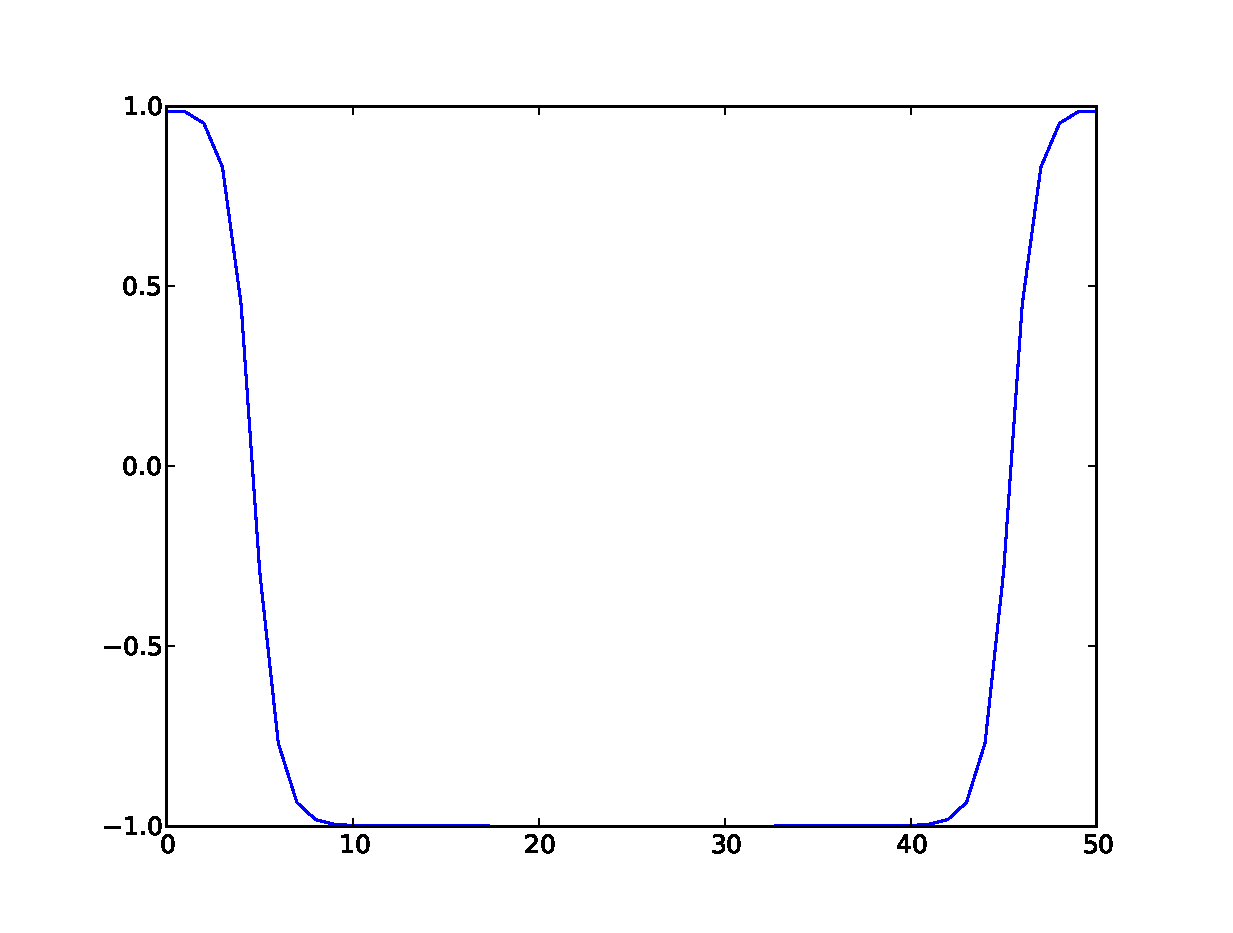
\includegraphics[width=0.47\textwidth]{Figures/plane_pressure_width_6.eps}
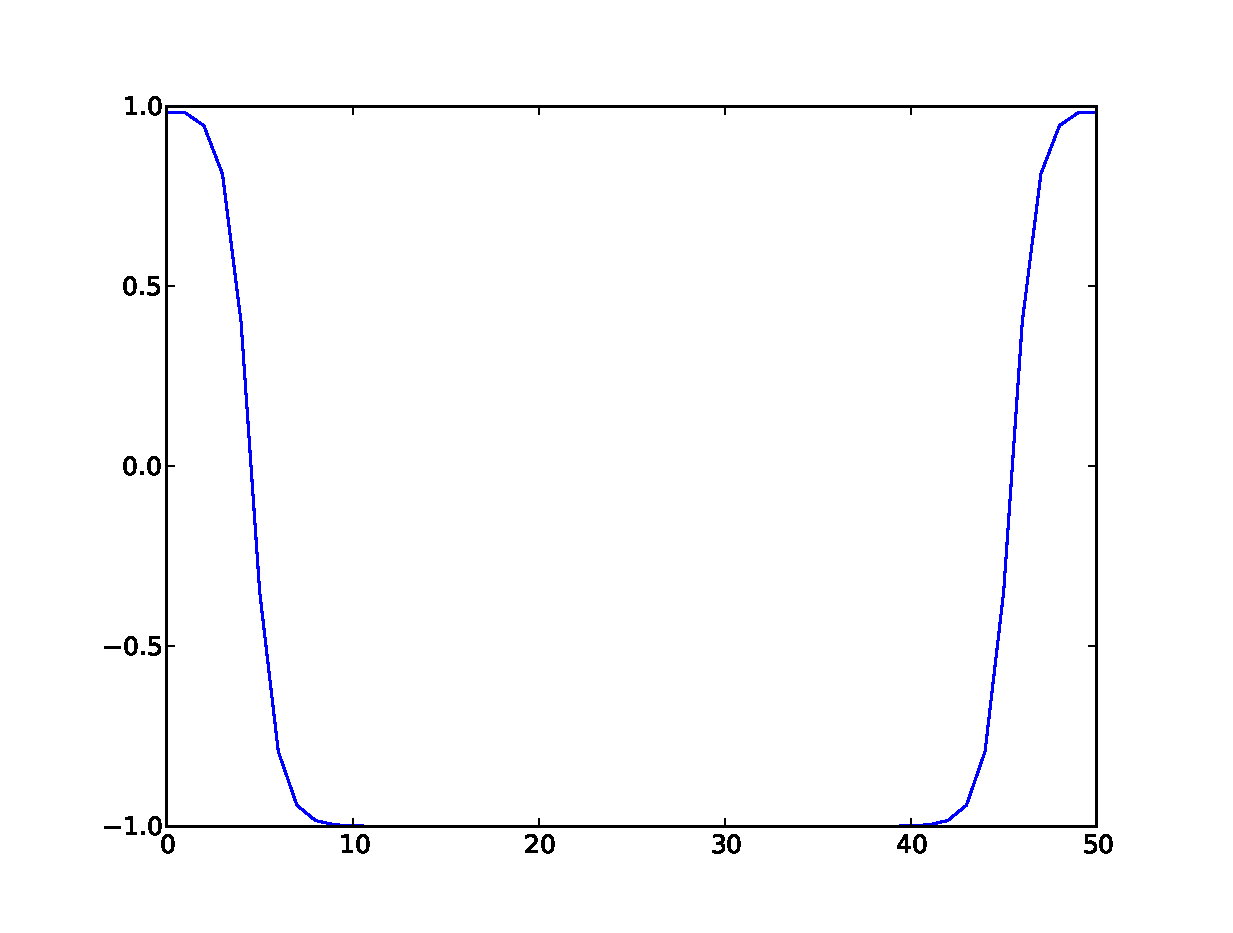
\includegraphics[width=0.47\textwidth]{Figures/plane_pressure_width_10.eps}
\begin{center}
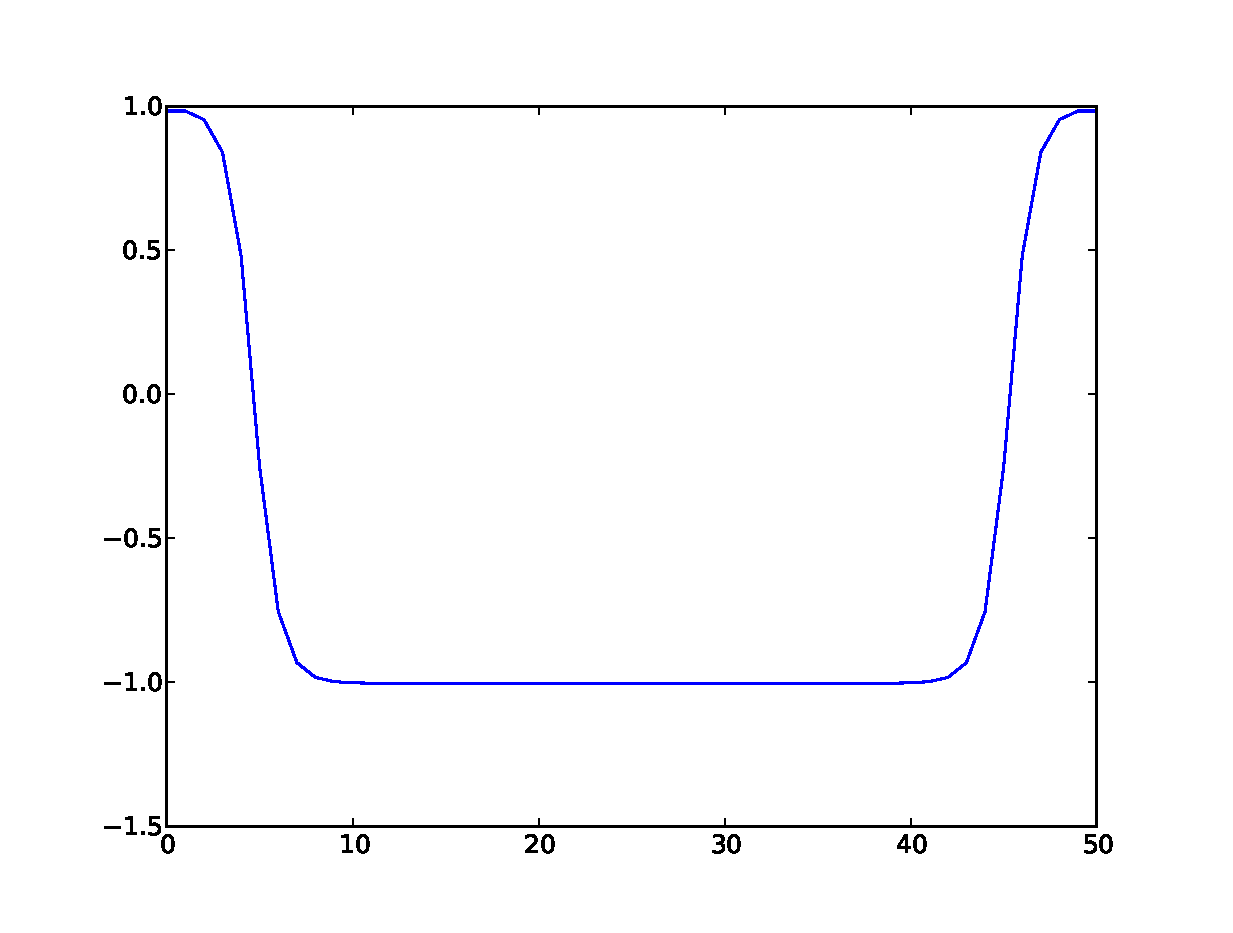
\includegraphics[width=0.47\textwidth]{Figures/plane_pressure_width_14.eps}
\end{center}
\caption{The phase profiles for different initialization parameters as the
bubble width $Ny-12$,$Ny-20$ and $Ny-28$.
\label{fig:phase:profiles:different:widths:pressure}}
\end{figure}
\begin{figure}
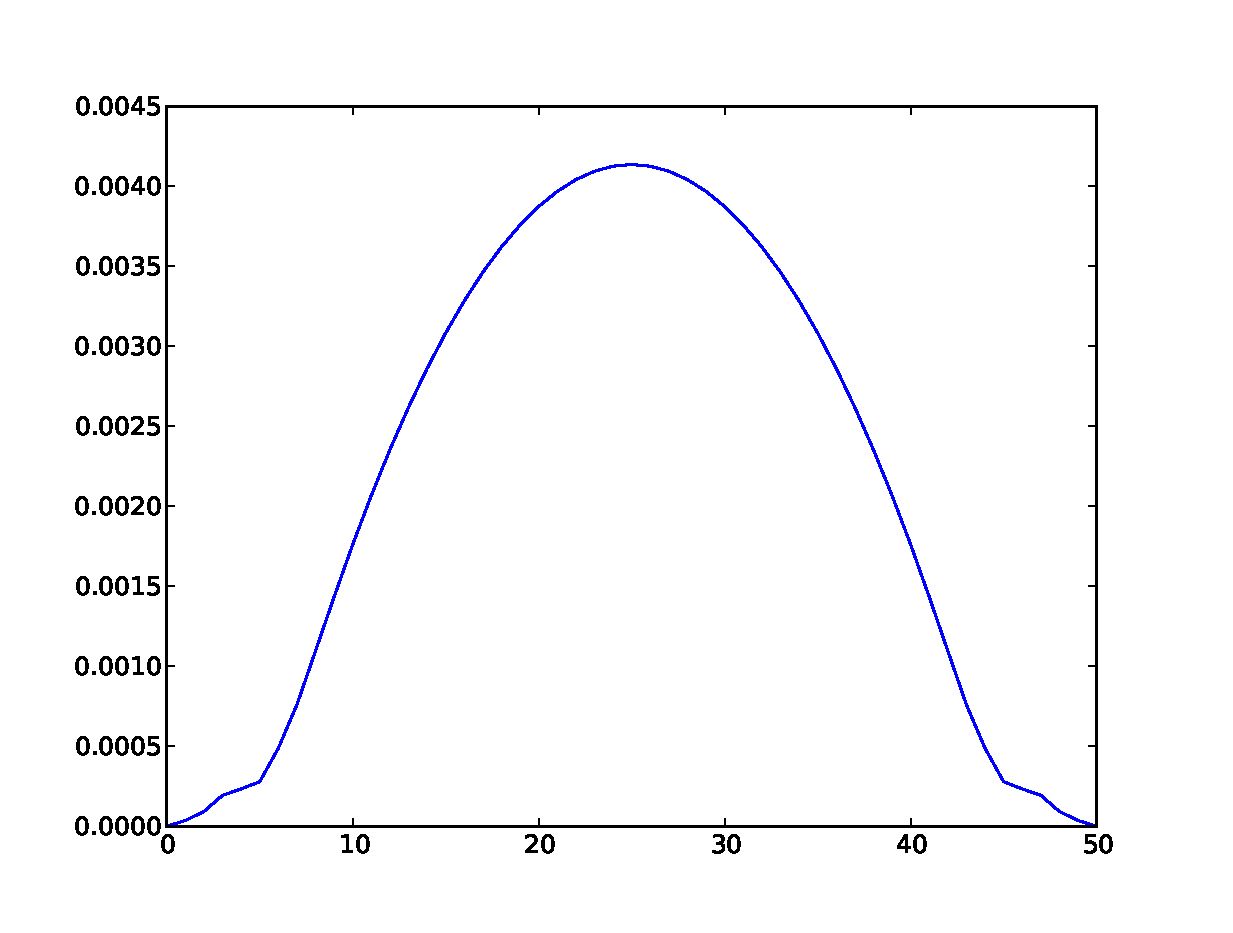
\includegraphics[width=0.47\textwidth]{Figures/vel_bubble_pressure_width_6.eps}
\hfill
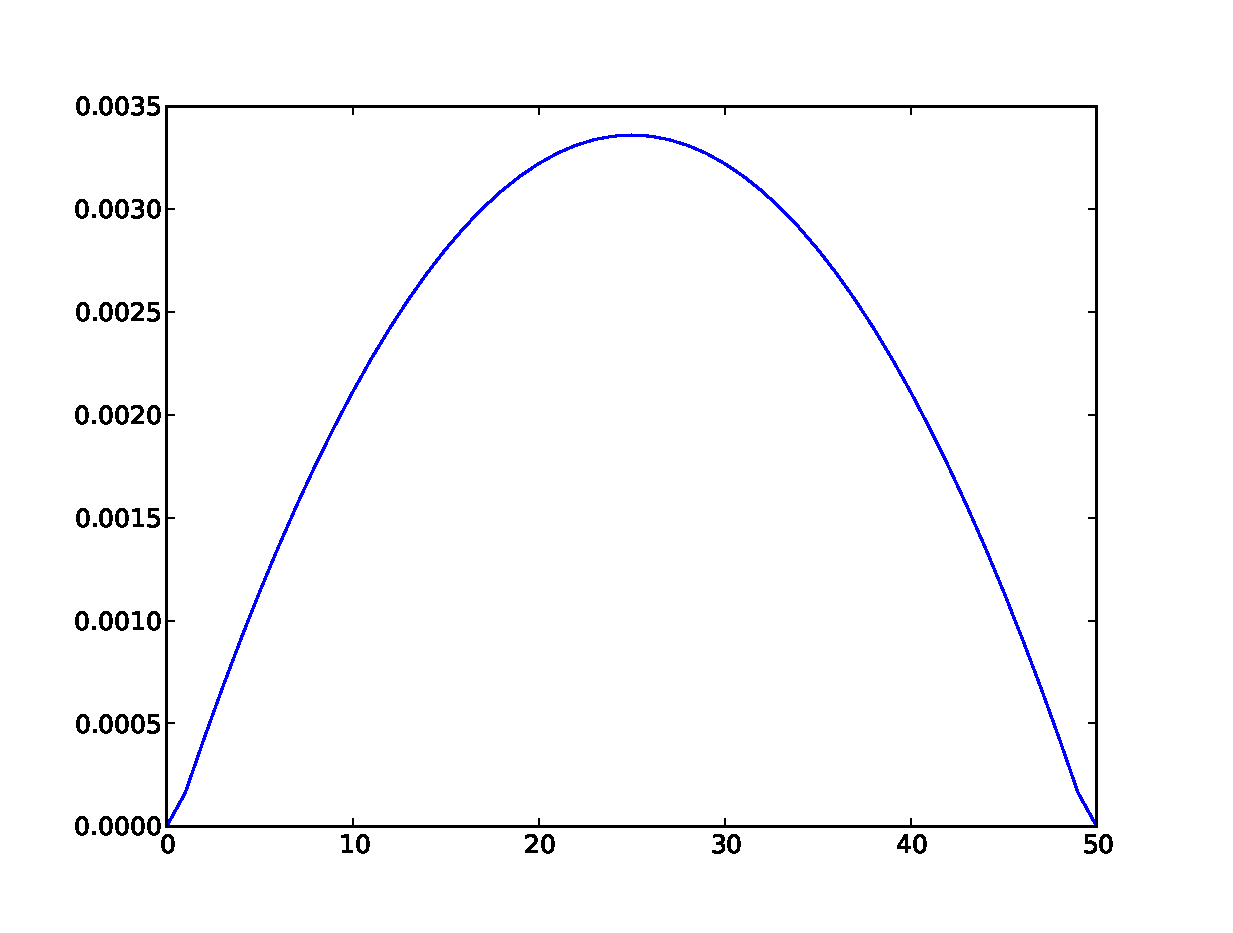
\includegraphics[width=0.47\textwidth]{Figures/vel_bulk_pressure_width_6.eps}\\
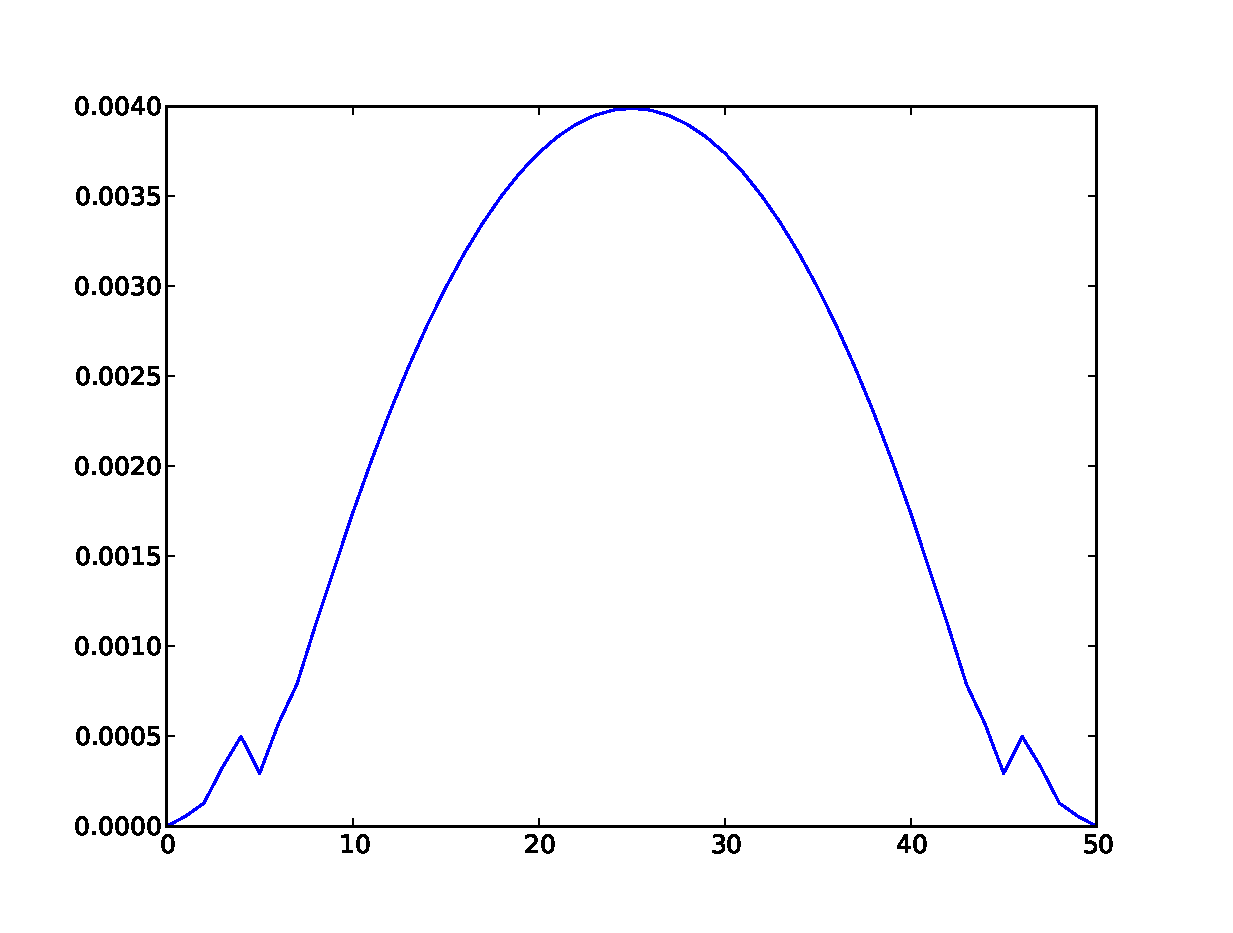
\includegraphics[width=0.47\textwidth]{Figures/vel_bubble_pressure_width_10.eps}
\hfill
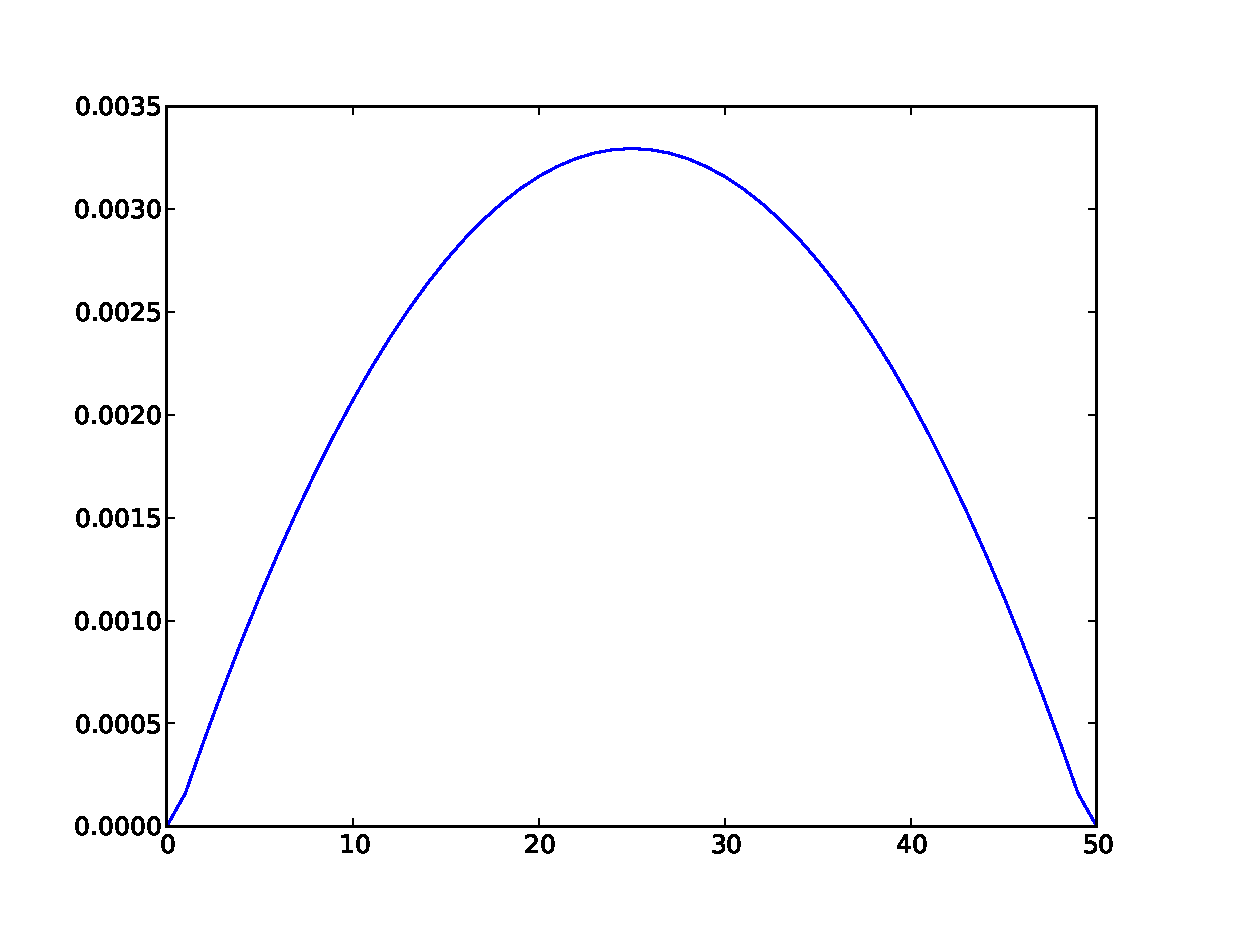
\includegraphics[width=0.47\textwidth]{Figures/vel_bulk_pressure_width_10.eps}\\
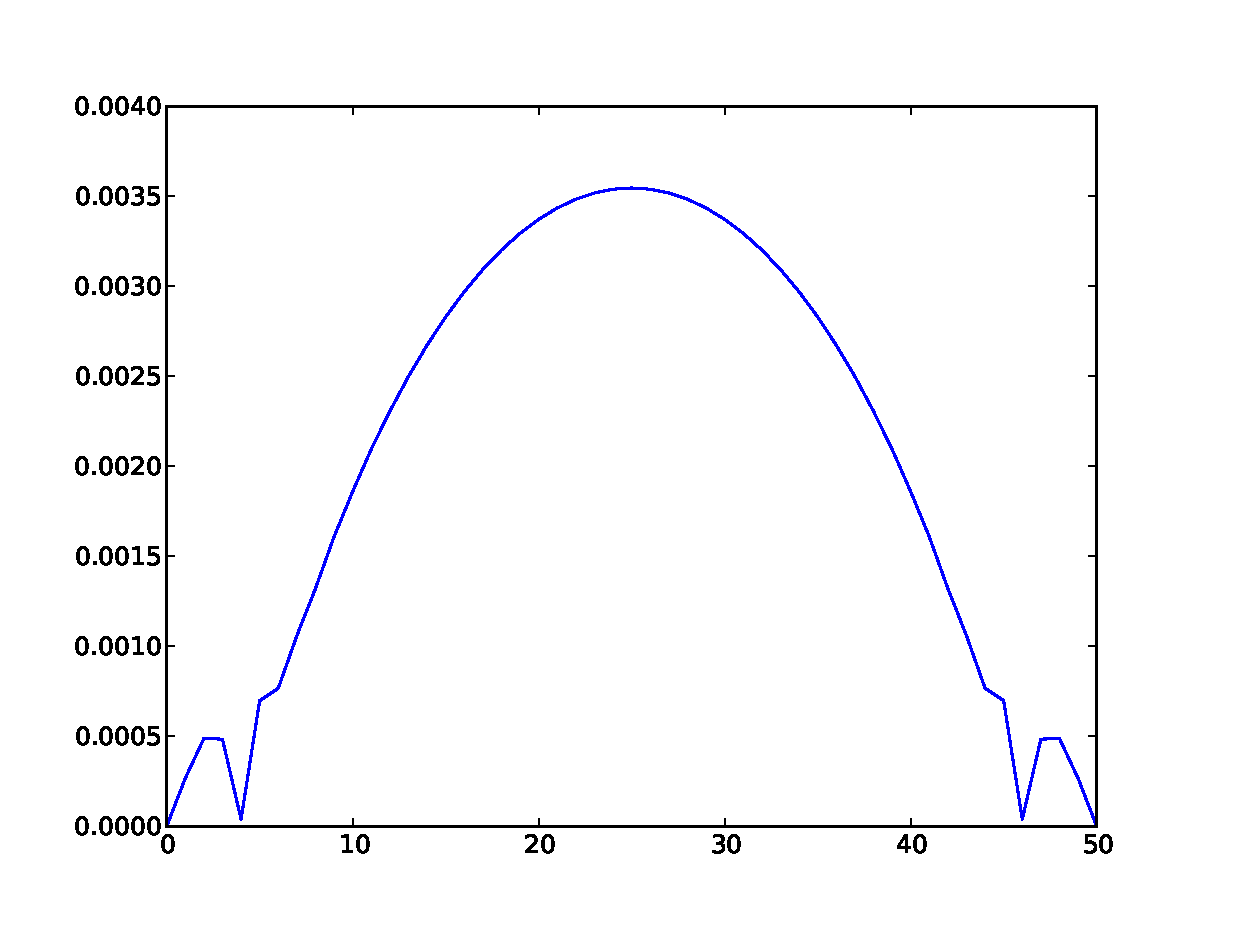
\includegraphics[width=0.47\textwidth]{Figures/vel_bubble_pressure_width_14.eps}
\hfill
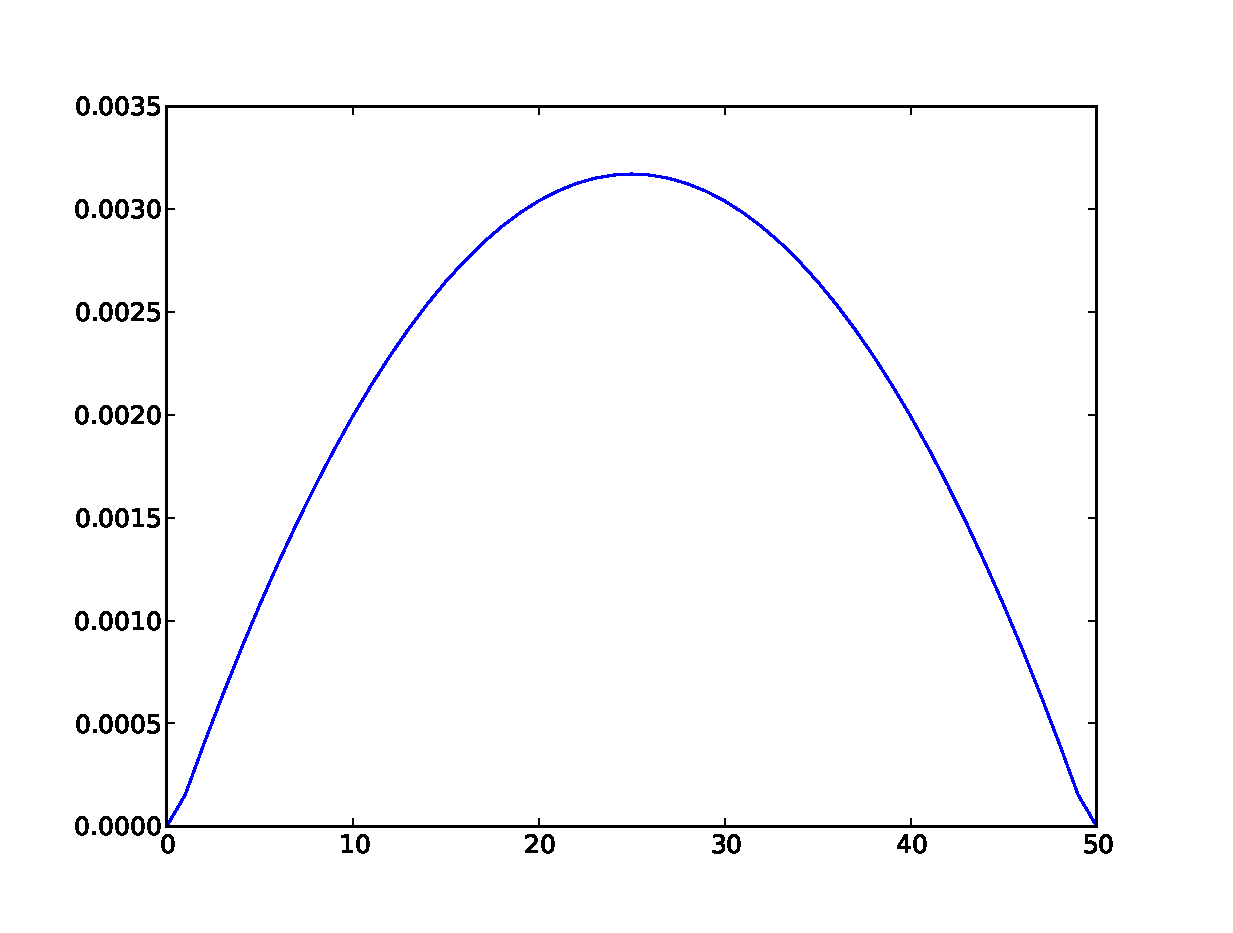
\includegraphics[width=0.47\textwidth]{Figures/vel_bulk_pressure_width_14.eps}\\
\caption{The velocity profiles in bulk and bubble for different initialization
parameters as the
bubble width $Ny-12$,$Ny-20$ and $Ny-28$.
\label{fig:velocity:profiles:different:widths:pressure}}
\end{figure}



\section{Appendix I. Pressure boundaries conditions}
\label{appendix-pressure}
Bulk pressure for the binary liquid model is a function not only of density
but the phase field as well. Thus, one of the possible ways to fix the pressure
boundary condition is to fix density and phase at the inleat and at the outlet.
The pressure difference is introduced through the difference in densities
keeping phases at the inlet and at the outlet the same. One can introduce the
pressure difference through the phase, however it's unphysical since the phase
field is governed by passive advection-diffusion equation, where velocity is
given from the hydrodynamic simulations.

We examined many different pressure boundaries conditions, including Zou-He BC
\cite{zouhe-boundary,harting-pressure}, equilibrium conditions for
the phase field, etc. However, the stable situation was obtained only with the
boundary conditions by \citeauthor{guo-pressure} \cite{guo-pressure,
guo-boundary-conditions}. The idea of the boundary conditions is simple: the
coming populations to domain are decomposed to the equilibrium and
non-equilibrium part:
\begin{equation}
f_i=f_i^{eq}(\rho_{wall},\bm{u}_{wall})+f_i^{neq}.
\end{equation}
The incoming population after the collision is changed due to collision:
\begin{equation}
f_i=f_i^{eq}(\rho_{wall},\bm{u}_{wall})+f_i^{neq} (1-\omega).
\end{equation}
The method is called extrapolation as the wall macroscopic parameters are
extrapolated from fluid using first or second accuracy numerical stencils. If
the pressure boundary condition is specified then it specifies $\rho_{wall}$ as
well extrapolating the wall velocity $\bm{u}_{wall}$ from nearest neighbours.
The same goes for the velocity boundary conditions, where velocity
$\bm{u}_{wall}$ is specified and $\rho_{wall}$ is extrapolated from the fluid.

It is pretty straightforward to obtain non-equilibrium contribution from the
fluid, however the equilibrium for the wall side needs special treatment. If
one wants to take the hydrodynamic equilibrium, the numerical scheme blows
up. Therefore, one needs to construct the equilibrium function as it's given
for the binary liquid model. The binary liquid model equilibrium contains local
density, local phase and phase laplacians and gradients. The pressure boundary
conditions specify the local phase and the local density. Therefore, we
extrapolate not only velocity to construct the equilibrium, but phase laplacian
and gradients. This situation produces stable simulations to be validated in
the future. 
\bibliographystyle{plainnat}
\bibliography{paper}

\end{document}
